\documentclass[a4paper,11pt]{article}
%----------------------------------------------------------------------------------------
%	COLOR SETUP
%----------------------------------------------------------------------------------------
%% Color package %%
\usepackage{xcolor}

%% Plots %%
\definecolor{carnelian}{rgb}{0.7, 0.11, 0.11}
\definecolor{Prune}{RGB}{99,0,60}

%% Orange
\definecolor{burntorange}{rgb}{0.8, 0.33, 0.0}
\definecolor{mahogany}{rgb}{0.75, 0.25, 0.0}

%% Pink
\definecolor{deepcarminepink}{rgb}{0.94, 0.19, 0.22}
\definecolor{dogwoodrose}{rgb}{0.84, 0.09, 0.41}
\definecolor{byzantine}{rgb}{0.74, 0.2, 0.64}

%% Beautiful Dark red:
\definecolor{carmine}{rgb}{0.59, 0.0, 0.09}

%% Yellow
\definecolor{amber}{rgb}{1.0, 0.75, 0.0}
\definecolor{mikadoyellow}{rgb}{1.0, 0.77, 0.05}
\definecolor{tangerineyellow}{rgb}{1.0, 0.8, 0.0}
\definecolor{mikadoyellow}{rgb}{1.0, 0.77, 0.05}

%% Blue
\definecolor{blue(munsell)}{rgb}{0.0, 0.5, 0.69}
\definecolor{yaleblue}{rgb}{0.06, 0.3, 0.57}
\definecolor{richelectricblue}{rgb}{0.03, 0.57, 0.82}
\definecolor{frenchblue}{rgb}{0.0, 0.45, 0.73}
\definecolor{steelblue}{rgb}{0.27, 0.51, 0.71}
\definecolor{skobeloff}{rgb}{0.0, 0.48, 0.45}

%% Green
\definecolor{yellow-green}{rgb}{0.6, 0.8, 0.2}
\definecolor{applegreen}{rgb}{0.55, 0.71, 0.0}
\definecolor{ballblue}{rgb}{0.13, 0.67, 0.8}

%% Dark Blue
\definecolor{indigo(dye)}{rgb}{0.0, 0.25, 0.42}
\definecolor{prussianblue}{rgb}{0.0, 0.19, 0.33}
\definecolor{darkmidnightblue}{rgb}{0.0, 0.2, 0.4}

%% Teal
\definecolor{tealgreen}{rgb}{0.0, 0.51, 0.5}
\definecolor{tealgreenperso}{rgb}{0.0, 0.5, 0.5}
\definecolor{teal}{rgb}{0.0, 0.5, 0.5}

\definecolor{arsenic}{rgb}{0.23, 0.27, 0.29}
\definecolor{coolblack}{rgb}{0.0, 0.18, 0.39}
\definecolor{gray}{gray}{0.55}

%% Sections, titles
\newcommand{\colortitle}{mahogany}
%burntorange, mahogany
\newcommand{\colorchapternumber}{\colorchapter}
\newcommand{\colorpartnumber}{\colorchapter}
\newcommand{\colorpart}{\colortitle}
\newcommand{\colorsubpart}{\colortitle}

\newcommand{\colorchapter}{indigo(dye)}
%indigo(dye), darkmidnightblue, prussianblue
\newcommand{\colorsubtitle}{\colorchapter}
\newcommand{\colorsection}{\colorchapter!92!white}
\newcommand{\colorsubsection}{\colorchapter!82!white}

\newcommand\myshade{85}
\newcommand{\colorurl}{byzantine!95!black}
\newcommand{\colorcite}{tealgreenperso!95!black}
\newcommand{\colorlink}{tangerineyellow!85!black}

\newcommand{\colorsubsubsection}{black}
\newcommand{\colorparagraph}{black}
\newcommand{\colorkeyword}{black}
\newcommand{\colorpage}{black}
\newcommand{\colorcomment}{black}

\usepackage{import} % sub levels import

%% Language and encoding %%
\PassOptionsToPackage{utf8}{inputenc}
\usepackage{inputenc}
\PassOptionsToPackage{french,american,english,british}{babel} 
\usepackage{babel}
\selectlanguage{french}
\usepackage{mathptmx}
\usepackage{tocloft}

%% Font %%
\PassOptionsToPackage{T1}{fontenc} % T2A for cyrillics
\usepackage{fontenc}
\usepackage{textcomp} % Fix warning with missing font shapes
\usepackage{scrhack} % Fix warnings when using KOMA with listings package  
\usepackage{xspace} % To get the spacing after macros right
\usepackage{mparhack} % To get marginpar right
\usepackage{fixltx2e} % Fixes some LaTeX stuff 
\PassOptionsToPackage{smaller}{acronym} 
\usepackage[printonlyused]{acronym}
% Acronym, option: [printonlyused]
\renewcommand*{\aclabelfont}[1]{\acsfont{#1}}
%% Different fonts
\usepackage[osf]{libertine}

%% Math %%
\PassOptionsToPackage{fleqn}{amsmath} % Math environments and more by the AMS 
\usepackage{amsmath,amsfonts,amssymb,amsthm,mathrsfs, bm}
\usepackage{amscd,amsbsy,dsfont}
\usepackage{nicefrac}
\usepackage{microtype}      % microtypography
\usepackage{mathtools}
\usepackage{nicefrac}       % compact symbols for 1/2, etc.
\usepackage{stmaryrd} % Fancy letters

%% Scientific %%
\usepackage[intoc,english]{nomencl} % nomenclature
\makenomenclature
\usepackage{etoolbox}
\usepackage{physics}
\usepackage{tensor}
\usepackage{empheq}

%% Algos %%
\usepackage{algorithmic}
\usepackage{algorithm2e}
	
%% Graphicx %%
\PassOptionsToPackage{pdftex}{graphicx}
\usepackage{graphicx} 
\usepackage{epstopdf}

%% Floats: Tables, Figures AND Captions
%\usepackage{enumitem}
\usepackage{mdwlist}
\usepackage{tabularx} % Better tables
\usepackage{booktabs} % professional-quality tables
\setlength{\extrarowheight}{3pt} % Increase table row height
\newcommand{\tableheadline}[1]{\multicolumn{1}{c}{\spacedlowsmallcaps{#1}}}
\newcommand{\myfloatalign}{\centering} % To be used with each float for alignment
\usepackage{caption}
\captionsetup{font=small}
\usepackage{subcaption}
%\usepackage{subfig}
\usepackage{float}
\usepackage{cases}
\usepackage{pdfpages} % pdfpages
\usepackage{bookmark}
\usepackage{adjustbox}
\usepackage{blkarray}
%% Nomencalture %%
\usepackage{nomencl}
\makenomenclature


%% Hyper references %%
\hypersetup{
colorlinks=true, linktocpage=true, pdfstartpage=3, pdfstartview=FitV,
urlcolor=\colorurl, linkcolor=\colorlink, citecolor=\colorcite,
}
\usepackage{url}
\usepackage{hyperref}
\usepackage{xr} % Cross references

%% Other %%
\usepackage[most]{tcolorbox}

%% Tikz %%
\usepackage{tikz}
\usetikzlibrary{arrows}
\tikzset{middlearrow/.style={decoration={markings,mark= at position 0.5 with {\arrow{#1}} ,},postaction={decorate}}}
\newcommand{\midarrow}{\tikz \draw[-triangle 90] (0,0) -- +(.1,0);}
\usetikzlibrary{decorations.markings}
\usetikzlibrary{fit}
\usetikzlibrary{bayesnet}
\usepackage{pgfplots}
\usetikzlibrary{calc}
\usepackage{ifthen}
\usetikzlibrary{decorations.text}
\usetikzlibrary{decorations.pathmorphing}
\usetikzlibrary{decorations.markings}
\usetikzlibrary{shapes.geometric}
\usetikzlibrary{shapes}
\usepackage{pgfplotstable}
\usetikzlibrary{fadings,shapes.arrows,shadows}   
\usetikzlibrary{calc}

\usetikzlibrary{external}
\tikzexternalize[mode=list and make]
\tikzexternaldisable


\newcommand{\aclink}[1]{#1}
\newcommand{\ie}{i.\,e.~}
\newcommand{\eg}{e.\,g.~}
\newcommand{\Sec}{Sec.~}
\newcommand{\Part}{Part~}
\newcommand{\Chap}{Chap.~}
\newcommand{\App}{Appendix.~}
\newcommand{\Alg}{Algo.~}
\newcommand{\Fig}{Fig.~}
\newcommand{\Tab}{Table.~}
\newcommand{\Left}{(\textbf{Left})~}
\newcommand{\Right}{(\textbf{Right})~}
\newcommand{\Center}{(\textbf{Center})~}
\newcommand{\Leftn}{(\textbf{Left})}
\newcommand{\Rightn}{(\textbf{Right})}
\newcommand{\Centern}{(\textbf{Center})}
\newcommand{\Up}{(\textbf{Up})~}
\newcommand{\Down}{(\textbf{Down})~}


\def \({\left(}
\def \){\right)}
\def \[{\left[}
\def \]{\right]}
\newcommand{\nn}{\nonumber \\}
\newcommand{\tbf}[1]{{\textbf{#1}}}
\newcommand{\bsy}[1]{{\boldsymbol{#1}}}
\newcommand{\txt}[1]{\text{#1}}
\newcommand{\defeq}{\vcentcolon=}
\newcommand{\eqdef}{=\vcentcolon}
\newcommand{\cv}[1]{\underline{#1}}
\newcommand{\bQ}{{\textbf {Q}}}
\newcommand{\bq}{{\textbf {q}}}
\newcommand{\br}{{\textbf {r}}}
\newcommand{\bU}{{\textbf {U}}}
\newcommand{\bu}{{\textbf {u}}}
\newcommand{\bV}{{\mathbf {V}}}
\newcommand{\bF}{{\textbf {F}}}
\newcommand{\bY}{{\textbf {Y}}}
\newcommand{\bff}{{\textbf {f}}}
\newcommand{\bG}{{\textbf {G}}}
\newcommand{\bW}{{\textbf {W}}}
\newcommand{\bZ}{{\textbf {Z}}}
\newcommand{\bh}{{\textbf {h}}}
\newcommand{\bw}{{\textbf {w}}}
\newcommand{\bv}{{\textbf {v}}}
\newcommand{\bA}{{\textbf {A}}}
\newcommand{\bB}{{\textbf {B}}}
\newcommand{\bhx}{\hat {\textbf {x}}}
\newcommand{\bX}{{\textbf {X}}}
\newcommand{\bx}{{\textbf {x}}}
\newcommand{\bo}{{\textbf {o}}}
\newcommand{\by}{{\textbf {y}}}
\newcommand{\bz}{{\textbf {z}}}
\newcommand{\bl}{{\textbf {l}}}
\newcommand{\bs}{{\textbf {s}}}
\newcommand{\bS}{{\textbf {S}}}
\newcommand{\bc}{{\textbf {c}}}
\newcommand{\bk}{{\textbf {k}}}
\newcommand{\bR}{{\textbf {R}}}
%% Bold greek %%
\newcommand{\beps}{{\boldsymbol {\epsilon}}}
\newcommand{\bxigma}{{\boldsymbol{\Sigma}}}
\newcommand{\bxi}{{\boldsymbol{\xi}}}
\newcommand{\bgamma}{{\boldsymbol{\gamma}}}
\newcommand{\bGamma}{{\boldsymbol{\Gamma}}}
\newcommand{\bomega}{{\boldsymbol{\omega}}}
\newcommand{\boldeta}{{\boldsymbol{\eta}}}
\newcommand{\btheta}{{\boldsymbol{\theta}}}
\newcommand{\bphi}{{\boldsymbol{\phi}}}
\newcommand{\bchi}{{\boldsymbol{\chi}}}
\newcommand{\brho}{{\boldsymbol{\rho}}}
\newcommand{\bsigma}{{\boldsymbol{\sigma}}}
\newcommand{\bSigma}{{\boldsymbol{\Sigma}}}
\newcommand{\blambda}{{\boldsymbol{\lambda}}}
\newcommand{\bLambda}{{\boldsymbol{\Lambda}}}
\newcommand{\bDelta}{{\boldsymbol{\Delta}}}
\newcommand{\btau}{{\boldsymbol{\tau}}}
\newcommand{\bzero}{{\textbf{0}}}
\newcommand{\bmu}{{\boldsymbol{\mu}}}
\newcommand{\bepsilon}{{\boldsymbol{\epsilon}}}

%% Mathcal
\newcommand{\cC}{{\mathcal{C}}}
\newcommand{\cB}{{\mathcal{B}}}

\newcommand{\ba}{{\textbf {a}}}

\newcommand{\lab}[1]{\label{#1}}
\newcommand{\bxii}{{\boldsymbol{\xi}}}
\newcommand{\bre}{{\textbf {e}}}
\newcommand{\bytilde}{{\tilde{\textbf {y}}}}
\newcommand{\bxhat}{{\tilde{\textbf {x}}}}

\newcommand{\eps}{\varepsilon}
\newcommand{\calF}{\mathcal F}
\newcommand{\s}{\sigma}
\renewcommand{\d}{\mathrm{d}}
\newcommand{\D}{\mathrm{D}}
\newcommand{\e}{\text {e}}
\newcommand{\ds}{\Delta\sigma}
\newcommand{\hw}{h^{\textrm W}}
\newcommand{\sw}{\sigma^{\textrm W}}
\newcommand{\<}{\langle}
\renewcommand{\>}{\rangle}
\newcommand{\de}{\partial}
\newcommand{\la}{\langle}
\newcommand{\ra}{\rangle}
\newcommand{\eq}{\text{ eq}.~}
\newcommand{\ua}{\uparrow}
\newcommand{\da}{\downarrow}
\newcommand{\be}{\begin{equation}}
\newcommand{\ee}{\end{equation}}
\newcommand{\beqa}{\begin{eqnarray}}
\newcommand{\eeqa}{\end{eqnarray}}
\newcommand\smallO{
  \mathchoice
    {{\scriptstyle\mathcal{O}}}% \displaystyle
    {{\scriptstyle\mathcal{O}}}% \textstyle
    {{\scriptscriptstyle\mathcal{O}}}% \scriptstyle
    {\scalebox{.7}{$\scriptscriptstyle\mathcal{O}$}}%\scriptscriptstyle
  }
\newcommand{\bea}{\begin{align}}
\newcommand{\eea}{\end{align}}

%% Theorems %%
\newtheorem{theorem}{Theorem}[section]
\newtheorem{lemma}[theorem]{\textbf{Lemma}}
\newtheorem{thm}[theorem]{\textbf{Theorem}}
\newtheorem{remark}[theorem]{\textbf{Remark}}
\newtheorem{proposition}[theorem]{\textbf{Proposition}}
\newtheorem{corollary}[theorem]{\textbf{Corollary}}
\newtheorem{definition}[theorem]{\textbf{Definition}}

\DeclareMathOperator{\atanh}{atanh}
\DeclareMathAlphabet{\varmathbb}{U}{bbold}{m}{n}
\newcommand{\id}{\mathds{1}}
\newcommand{\EE}{\mathbb{E}}
\newcommand{\bbR}{\mathbb{R}}
\newcommand{\bbX}{\mathbb{X}}
\newcommand{\bbH}{\mathbb{H}}
\newcommand{\bbK}{\mathbb{K}}
\newcommand{\bbY}{\mathbb{Y}}
\newcommand{\bbD}{\mathbb{D}}
\newcommand{\bbS}{\mathbb{S}}
\newcommand{\bbT}{\mathbb{T}}
\newcommand{\bbP}{\mathbb{P}}
\newcommand{\bbZ}{\mathbb{Z}}
\newcommand{\bbN}{\mathbb{N}}
\newcommand{\bbM}{\mathbb{M}}
\newcommand{\bbA}{\mathbb{A}}
\newcommand{\bbB}{\mathbb{B}}
\newcommand{\bbQ}{\mathbb{Q}}
\newcommand{\bbC}{\mathbb{C}}
\newcommand{\bbV}{\mathbb{V}}
\renewcommand{\d}{{\mathrm d}}
\renewcommand{\P}{{\mathrm P}}
\newcommand{\B}{{\mathrm B}}
\newcommand{\iif}{\Longleftrightarrow}
\newcommand{\noi}{\noindent}

\def\du#1{\underline{\underline{#1}}}
\newcommand{\ud}[1]{{\underline{#1}}}
\newcommand{\mZ}{\mathcal{Z}}
\newcommand{\mH}{\mathcal{H}}
\newcommand{\mO}{\mathcal{O}}
\newcommand{\mI}{\mathcal{I}}
\newcommand{\mM}{\mathcal{M}}
\newcommand{\mN}{\mathcal{N}}
\newcommand{\mS}{\mathcal{S}}
\newcommand{\mC}{\mathcal{C}}
\newcommand{\mD}{\mathcal{D}}
\newcommand{\mX}{\mathcal{X}}
\newcommand{\mY}{\mathcal{Y}}
\newcommand{\mL}{\mathcal{L}}
\newcommand{\mA}{\mathcal{A}}
\newcommand{\mB}{\mathcal{B}}
\newcommand{\mR}{\mathcal{R}}
\newcommand{\mF}{\mathcal{F}}
\newcommand{\mG}{\mathcal{G}}
\newcommand{\mP}{\mathcal{P}}
\newcommand{\mQ}{\mathcal{Q}}
\newcommand{\mE}{\mathcal{E}}
\newcommand{\mT}{\mathcal{T}}
	
\renewcommand{\tr}[1]{\textrm{Tr}\(#1\)}
\renewcommand{\det}[1]{\textrm{det}\(#1\)}
\newcommand{\diag}[1]{\textrm{diag}\(#1\)}
\newcommand{\td}[1]{{\tilde{#1}}}
\newcommand{\cov}[1]{\textrm{Cov}\[#1\]}

\newcommand{\fixme}[1]{
{ \sffamily\normalsize\bfseries \color{red} \underline{FIXME \index{Fixme}:}
\rmfamily \normalsize #1.}\\}

\newcommand{\spacecase}[0]{\vspace{0.3cm} \\}
\newcommand{\Spacecase}[0]{\vspace{0.5cm} \\}
\newcommand{\hhspace}[0]{\hspace{0.3cm}}
\newcommand{\Eq}[1]{(Eq.#1)}

\def\E{\mathbb{E}}
\def\eps{\epsilon}
\def\del{\delta}
\def\cE{\mathcal E}
\newcommand{\Var}[1]{\textrm{Var}(#1)}


\newcommand{\andcase}[0]{\hspace{ 0.2cm }\textrm{ and }\hspace{ 0.2cm }}


\renewcommand{\vec}[1]{{\mathbf{#1}}}
\newcommand{\mat}[1]{{\mathbf{#1}}}

\newcommand{\erfc}{{\textrm erfc}}
\newcommand{\relu}{{\textrm{relu}}}
\newcommand{\sign}{{\textrm{sign}}}
\newcommand{\linear}{{\textrm{linear}}}

\newcommand{\W}[1]{{\mat{W}^{[#1]}}}
\newcommand{\Y}[0]{{\mat{Y}}}
\newcommand{\Z}{\mat{Z}}
\newcommand{\mW}[0]{{\mat{W}}}
\newcommand{\X}[0]{{\mat{X}}}
\renewcommand{\S}[0]{{\mat{S}}}
\newcommand{\R}[0]{{\mat{R}}}
\newcommand{\m}[0]{\mat{m}}
\newcommand{\q}[0]{\mat{q}}
\newcommand{\Q}[0]{\mat{Q}}
\newcommand{\mh}[0]{\hat{\mat{m}}}
\newcommand{\qh}[0]{\hat{\mat{q}}}
\newcommand{\Qh}[0]{\hat{\mat{Q}}}
\newcommand{\iid}[0]{{\textrm{iid}~}}
\newcommand{\out}[0]{\mathrm{out}}
\newcommand{\w}[0]{{\mathrm{w}}}
\renewcommand{\u}[0]{{\mathrm{u}}}
\renewcommand{\v}[0]{{\mathrm{v}}}
\newcommand{\z}[0]{{\mathrm{z}}}
\newcommand{\x}[0]{{\mathrm{x}}}
\newcommand{\y}[0]{{\mathrm{y}}}

\newcommand{\rI}[0]{\mat{I}}
\newcommand{\rJ}[0]{\mat{J}}
\newcommand{\rB}[0]{{\mathrm{B}}}
\newcommand{\rC}[0]{{\mathrm{C}}}
\newcommand{\rH}[0]{{\mathrm{H}}}
\newcommand{\rU}[0]{{\mathrm{U}}}
\newcommand{\rS}[0]{{\mathrm{S}}}
\newcommand{\rP}[0]{{\mathrm{P}}}
\newcommand{\rG}[0]{{\mathrm{G}}}
\newcommand{\rQ}[0]{{\mathrm{Q}}}
\newcommand{\rE}[0]{{\mathrm{E}}}
\newcommand{\rV}[0]{{\mathrm{V}}}
\newcommand{\rF}[0]{{\mathrm{F}}}
\newcommand{\bg }[0]{{\textbf{g}}}
\newcommand{\rp}[0]{{\mathrm{p}}}
\renewcommand{\rq}[0]{{\mathrm{q}}}
\newcommand{\rg}[0]{{\mathrm{g}}}
\newcommand{\rd}[0]{{\mathrm{d}}}
\newcommand{\rX}[0]{{\mathrm{X}}}
\newcommand{\rY}[0]{{\mathrm{Y}}}


\newcommand{\underlim}[2]{\underset{#1 \to #2}{\longrightarrow}}
\newcommand{\extr}{{\textbf{extr}}}
\newcommand{\Diff}{\mathrm{D}}
\newcommand{\argmin}{\mathrm{argmin}}
\newcommand{\argmax}{\mathrm{argmax}}
\newcommand{\train}{\mathrm{train}}
\newcommand{\test}{\mathrm{test}}
\newcommand{\MSE}{\mathrm{MSE}}
\newcommand{\gs}{\mathrm{gs}}
\newcommand{\bayes}{\mathrm{b}}
\newcommand{\gibbs}{\mathrm{gibbs}}
\newcommand{\vc}{\mathrm{vc}}
\newcommand{\mmse}{\mathrm{mmse}}
\newcommand{\map}{\mathrm{map}}
\newcommand{\mle}{\mathrm{mle}}
\newcommand{\rL}[0]{{\ell}}
\newcommand{\gen}{\mathrm{gen}}
\newcommand{\rs}{\mathrm{rs}}
%\newcommand{\1rsb}{1\mathrm{rsb}}
%\newcommand{\2rsb}{2\mathrm{rsb}}


%% Color boxes %%

\definecolor{green}{RGB}{0, 153, 0}
\definecolor{light_blue}{RGB}{51, 153, 255}
\definecolor{orange}{RGB}{255, 204, 0}
\definecolor{bg}{RGB}{0, 153, 153}
\definecolor{blue}{RGB}{0, 102, 204}
\definecolor{red}{RGB}{204, 0, 0}
\definecolor{lg}{RGB}{214, 214, 214}

\renewcommand{\colorbox}[1]{\fcolorbox{lg}{lg}{
\begin{minipage}{0.8\linewidth}
#1
\end{minipage}} }


\newcommand{\boxedred}[1]{\textcolor{red}{%
\tikz[baseline={([yshift=-1ex]current bounding box.center)}] \node [rectangle,line width=1.5, minimum width=1ex,draw] {\normalcolor$\displaystyle#1$};}}
\newcommand{\boxedblack}[1]{\textcolor{black}{%
\tikz[baseline={([yshift=-1ex]current bounding box.center)}] \node [rectangle,line width=1.5, minimum width=1ex,draw] {\normalcolor$\displaystyle#1$};}}
\newcommand{\boxedorange}[1]{\textcolor{BurntOrange}{%
\tikz[baseline={([yshift=-1ex]current bounding box.center)}] \node [rectangle,line width=1.5, minimum width=1ex,draw] {\normalcolor$\displaystyle#1$};}}
\newcommand{\boxedteal}[1]{\textcolor{teal}{%
\tikz[baseline={([yshift=-1ex]current bounding box.center)}] \node [rectangle,line width=1.5, minimum width=1ex,draw] {\normalcolor$\displaystyle#1$};}}
\newcommand{\boxedgreen}[1]{\textcolor{ForestGreen}{%
\tikz[baseline={([yshift=-1ex]current bounding box.center)}] \node [rectangle,line width=1.5, minimum width=1ex,draw] {\normalcolor$\displaystyle#1$};}}

\newcommand{\idea}[2]{{\color{yellow} \Large \faLightbulbO} \hspace{0.3cm} \textbf{#1} {#2}}

\newcommand{\tod}[2]{{\color{red} \faFlagCheckered} \hspace{0.3cm} \textbf{#1} {#2}}

\newcommand{\run}[2]{{\color{orange} \faHourglassStart} \hspace{0.3cm} \textbf{#1} {#2}}

\newcommand{\done}[2]{{\color{green} \faCheck} \hspace{0.3cm} \textbf{#1} {#2}}

\definecolor{codegreen}{rgb}{0,0.6,0}
\definecolor{codegray}{rgb}{0.5,0.5,0.5}
\definecolor{codepurple}{rgb}{0.58,0,0.82}
\definecolor{backcolour}{rgb}{0.95,0.95,0.92}
\lstdefinestyle{mystyle}{
    backgroundcolor=\color{backcolour},   
    stringstyle=\color{codepurple},
    commentstyle=\color{codegreen},
    numberstyle=\tiny\color{codegray},
    basicstyle=\ttfamily\footnotesize,
    numbers=left,      
}
\lstset{style=mystyle}


\newcommand*{\colorboxed}{}
\def\colorboxed#1#{%
  \colorboxedAux{#1}%
}
\newcommand*{\colorboxedAux}[3]{%
  % #1: optional argument for color model
  % #2: color specification
  % #3: formula
  \begingroup
    \colorlet{cb@saved}{.}%
    \color#1{#2}%
       \boxed{%
      \color{cb@saved}%
      #3%
    }%
  \endgroup
}

\renewcommand{\boxed}[1]{
\tikz[baseline={([yshift=-1ex]current bounding box.center)}] \node [rectangle,line width=1.25, minimum width=1ex,draw, color=red] {\normalcolor $\displaystyle#1$};}
 \makeatother
  
\newtheorem{prop}[theorem]{Proposition}
\newtheorem{conjecture}[theorem]{Conjecture}
\newtheorem{hypothesis}[theorem]{Hypothesis}
\newtheorem{assumption}[theorem]{Assumption}
\theoremstyle{remark}
\newtheorem*{remark*}{\textbf{Remark}}

 \newenvironment{proofof}[1]{{\bf {\em Proof of #1.}}}{\hfill \rule{2mm}{2mm} %\qed 
 }
 
\def\E{\mathbb{E}}
\def\eps{\epsilon}
\def\del{\delta}
\def\cE{\mathcal E}

\def\T{\text{T}}
\def\out{\text{out}}
\def\x{\text{x}}
\def\DD{\text{D}}
\def\spam{\text{spam}}
\def\dd{\text{d}}
\def\MSE{\text{MSE}}
\def\MMSE{\text{MMSE}}
\def\IT{\text{IT}}
\def\alg{\text{alg}}
\def\sign{\text{sign}}
\def\PR{\text{PR}}
\def\extr{{  \textbf{extr}}}
\def\erf{\text{erf}}
\def\erfc{\text{erfc}}

\newcommand{\KL}{\textrm{KL}}
\newcommand{\tramp}{\textsf{tramp}\xspace}
\newcommand{\lasso}{\textsf{LASSO}\xspace}
\newcommand{\pymc}{\textsf{PyMC3}\xspace}
\newcommand{\scikit}{\textsf{Scikit-Learn}\xspace}

% Single braces
\newcommand{\agbrs}[1]{\left\langle #1 \right\rangle}
\newcommand{\rdbrs}[1]{\left( #1 \right)}	
\newcommand{\sqbrs}[1]{\left\lbrack #1 \right\rbrack}
\newcommand{\clbrs}[1]{\left\lbrace #1 \right\rbrace}

\def\T{\text{T}}
\def\DD{\text{D}}
\def\dd{\text{d}}
\def\MSE{\text{MSE}}
\def\MMSE{\text{MMSE}}
\def\eff{\text{eff}}

\newcommand{\lb}{\llbracket}
\newcommand{\rb}{\rrbracket}
\newcommand{\intbracket}[1]{\lb #1 \rb}

%% Scale math
\newcommand\scalemath[2]{\scalebox{#1}{\mbox{\ensuremath{\displaystyle #2}}}}

\usetikzlibrary{decorations.text}
\tikzstyle{var}=[circle, draw, very thick, minimum size=12pt, inner sep=0pt, fill=burntorange, font=\small]
\tikzstyle{inter}=[rectangle, draw, very thick, minimum size=12pt, inner sep=0pt, fill=teal, font=\small]
\tikzstyle{field}=[rectangle, draw, very thick, minimum size=12pt, inner sep=0pt, fill=amber, font=\small]
\tikzstyle{fun}=[rectangle, draw, very thick, minimum size=15pt, inner sep=0pt, fill=teal]
\tikzstyle{edge} = [draw, thick, -]
\newcommand{\AxisRotator}[1][rotate=0]{%
    \tikz [x=0.25cm,y=0.60cm,line width=.2ex,-stealth,#1, dashed] \draw (0,0) arc (-150:150:1 and 1);%
}
\newcommand{\arcarrow}[8]{
  \pgfmathsetmacro{\rin}{#1}
  \pgfmathsetmacro{\rmid}{#2}
  \pgfmathsetmacro{\rout}{#3}
  \pgfmathsetmacro{\astart}{#4}
  \pgfmathsetmacro{\aend}{#5}
  \pgfmathsetmacro{\atip}{#6}
  \fill[#7] (\astart:\rin) arc (\astart:\aend:\rin)
       -- (\aend+\atip:\rmid) -- (\aend:\rout) arc (\aend:\astart:\rout)
       -- (\astart+\atip:\rmid) -- cycle;
  \path[decoration = {text along path, text = {#8},
    text align = {align = center}, raise = -0.5ex}, decorate]
    (\astart+\atip:\rmid) arc (\astart+\atip:\aend+\atip:\rmid);
}

\newcommand\randompath[2]{%
\pgfmathsetseed{#1}%
\addplot[#2,domain=0:1,samples=100,smooth] { x+rand*(x)*(1-x)};%
}

\tikzset{My Arrow Style/.style={single arrow, fill=red!50, anchor=base, align=center,text width=2.8cm}}
\newcommand{\MyArrow}[4][]{\tikz[baseline] \node [My Arrow Style,#1] {#2};}

\begin{document}

\title{\huge Tutorial: Approximate Message Passing \& Replicas for committee machines}
\author{Benjamin Aubin$^\dagger$}
\date{
$\dagger$ \textit{Institut de Physique Th\'eorique \\
CNRS \& CEA \& Universit\'e Paris-Saclay, Saclay, France}\\
}

\maketitle
\makeatletter
\tableofcontents
\newpage

%% Global notations %%
\newcommand{\ndim}{d}
\newcommand{\nsamples}{n}
\newcommand{\indsamples}{\mu}
\newcommand{\inddim}{i}

%% Main %%
\section{Introduction}

The purpose of these notes is to provide a short introduction to \textbf{Approximate Message Passing (AMP) algorithms} and \textbf{replicas} computation, that we illustrate for \textbf{committee machines}, that are a simple generalization of \textbf{generalized linear models}. For more details, see in particular the references \cite{mezard1987spin, Castellani2005, Barbier2017b, Yedidia2001, Krzakala2012, Zdeborova2016, Lesieur2017}.


\subsection{Model}

We revisit the so-called \emph{teacher-student} scenario from statistical physics \cite{Patarnello_1987,gardner1989three,tishby89,Sompolinsky1990,seung1992statistical,watkin1993statistical,Gyorgyi2001}. 
We assume that the synthetic dataset is generated by a \emph{teacher} model. 

\subsubsection{Data}

We assume that the matrix of data inputs $\mat{X} \in \bbR^{\nsamples \times \ndim }$, that contains $\nsamples$ $\ndim$-dimensional samples, is drawn \aclink{i.i.d} with distribution $\rP_\x(\mat{X}) = \displaystyle \prod_{i,\mu=1}^{\ndim, \nsamples} \rP_\x(x_{\mu i})$.\\
For simplicity, we will consider them to be \aclink{i.i.d} Gaussian with zero mean and unit variance: $\forall \mu \in \lb \nsamples \rb, \vec{x}_{\mu} \sim \mN_{\vec{x}}\(\vec{0}, \mat{I}_{\ndim}\)$.

\subsubsection{Teacher - Planted solution}
Moreover, we draw a \textbf{planted solution} $\mat{W}^\star$ from a separable distribution (across the input dimension) $\rP_{\w^\star}(\mat{W}^\star) = \prod_{i=1}^\ndim \rP_{\w^\star}\(\vec{w}_i^\star\)$. Therefore the weights could possibly be correlated across the second dimension.


\begin{figure}[htb!]
\centering
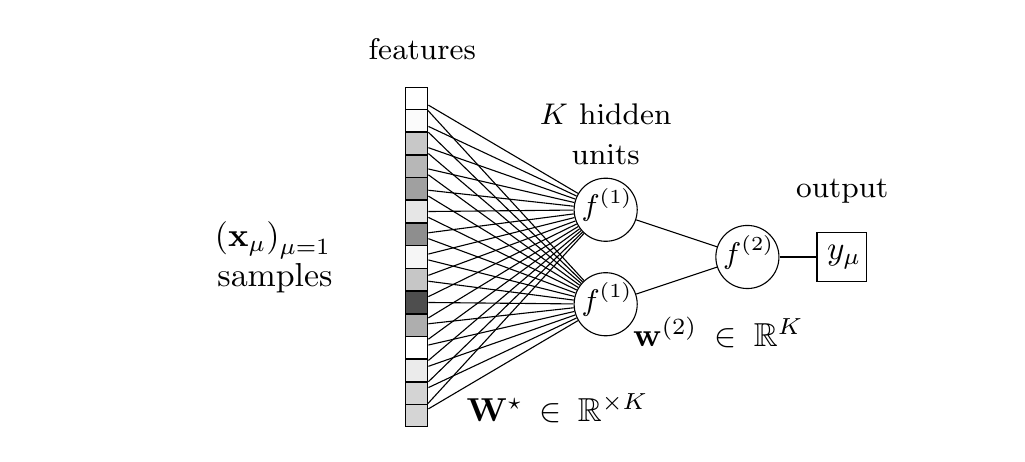
\begin{tikzpicture}[scale=1.2, every node/.style={transform shape}]
    \tikzstyle{factor}=[rectangle,minimum size=4pt,draw=black, fill opacity=1.]
    \tikzstyle{latent}=[circle,minimum size=19pt,draw=black, fill opacity=1.,fill=white]
    \tikzstyle{output}=[circle,minimum size=19pt,draw=black, fill opacity=1.,fill=white]
        \tikzstyle{noise}=[circle,minimum size=18pt,draw=black, fill opacity=1.,fill=white]
    \tikzstyle{output_y}=[rectangle,minimum size=15pt,draw=black, fill opacity=1.,fill=white]
    \tikzstyle{annot} = [text width=3cm, text centered]
    \tikzstyle{annot} = [text width=3cm, text centered]
    \tikzstyle{annotLarge} = [text width=5cm, text centered]
    \def\NX{15}
    \def\NK{2}
    \def\NY{1}
    \def\middle{0}
    \foreach \i in {1,...,\NX}
     	  \pgfmathparse{0.9*rnd+0.3}
          \definecolor{MyColor}{rgb}{\pgfmathresult,\pgfmathresult,\pgfmathresult}
    	\node[factor, fill=MyColor] (X-\i) at (\middle 0, 0.24*0.5*\NX+0.12 - 0.24*\i ) {}; 
    \foreach \k in {1,...,\NK}
    	\node[latent] (K-\k) at (2,\middle  \k - 1.5) {}; 
    \foreach \y in {1,...,\NY}
    	\node[output] (Y-\y) at (3.5,0) {}; 	
    \node[output_y] (Y-2) at (4.5,0) {}; 
    
    \foreach \i in {1,...,\NX}
    	\foreach \k in {1,...,\NK}
    		\path[-] (X-\i) edge (K-\k);
   	\foreach \k in {1,...,\NK}
    	\foreach \y in {1,...,\NY}
    		\path[-] (K-\k) edge (Y-\y);
    \path[-] (Y-1) edge (Y-2);
    \node[annotLarge] at (-1.5,0) {$(\vec{x}_{\mu})_{\mu=1}^{\nsamples}$ \\ samples};
    \node[annot] at (1.5,-1.6) {$\mat{W}^\star \in \bbR^{\ndim \times K}$}  ;
    \node[annot] at (4.525,0) {${y_{\mu}}$}  ;
    \node[annot] at (3.2,-0.8) {$\vec{w}^{(2)}\in\bbR^{K}$}  ;
    \node[annot] at (2,-0.45) {\small $ f^{(1)}$}  ;
    \node[annot] at (2,0.55) {\small $ f^{(1)}$}  ;
    \node[annot] at (3.5,0.05) {\small $ f^{(2)}$}  ;
    \node[annot] at (0,2.2) {\small $\ndim$ features}  ;
    \node[annot] at (2,1.3) {\small $K$ hidden\\ units}  ;
    \node[annot] at (4.5,0.7) {\small output}  ;
	\end{tikzpicture}	
	\caption{Illustration of the \emph{committee machine}: it is one of the simplest models belonging to the considered model class \eqref{model}, and on which we focus to illustrate our results. It is a two-layers neural network with sign activation functions $f^{(1)},f^{(2)}=\sign$ and weights $\vec{w}^{(2)}$ fixed to unity. It is represented for $K=2$.}
	\label{fig:committee}
\end{figure}


\subsubsection{Channel}

The labels are then generated by multiplying the data matrix $\mat{X}$ and the planted weights $\mat{W}^\star$ and passing their product to a \textbf{channel} $\varphi_\out$, acting component-wise, according to:

\begin{equation}
\label{model}
\vec{y} = \varphi_\out \( \left\{ \frac{1}{\sqrt{\ndim}} \mat{X} \vec{w}_k^\star \right \}_{k=1}^K \) ~~~\text{or}~~~ \vec{y} \sim \rP_\out \( \cdot \Big| \left\{ \frac{1}{\sqrt{\ndim}} \mat{X} \vec{w}_k^\star \right \}_{k=1}^K \)\, ,
\end{equation}
and illustrated in \Fig\ref{fig:committee} in the case of a committee machine with fixed weights $\vec{w}^{(2)}$ in the second layer.

The function $\varphi_\out : \bbR^{K} \mapsto \bbR$ represents a deterministic, or stochastic function associated to a probability distribution $\rP_\out$, applied component-wise to each sample. 

\begin{remark}
	Notice that the factor $\frac{1}{\sqrt{\ndim}}$ is present to insure that the variance of the input data is normalized to the unit.
\end{remark}


\subsubsection{Student}

The committee machine estimation problem consists of trying to fit the $\nsamples$ input-output observations $\{\mat{X}, \vec{y} \}\in \bbR^{\nsamples \times \ndim} \times \bbR^{\nsamples}$.\\

In the case the \textbf{student} has exactly the same architecture, namely $\mat{W}^\star \in \bbR^{\ndim \times K}$ and $\mat{W} \in \bbR^{\ndim \times K}$ have the same dimensionality and prior information $\rP_{\w^\star}=\rP_{\w}$, this setting is called the \textbf{Bayes-optimal setting}. Otherwise, it is called the \textbf{mismatched setting}.\\

In these notes, we focus on the \textbf{Bayes-optimal setting}, so that the committee machine estimation problem for the student committee machine (within the same hypothesis class and with weights $\mat{W}\in \bbR^{\ndim \times K}$) reduces to learn the teacher rule generated by the ground truth weights $\mat{W}^\star$ from the supervised dataset $\{\mat{X}, \vec{y} \}$.

\begin{remark}
	Committee machines are a simple vectorized generalization of \textbf{GLM}, whose estimation is performed simultaneously with $K \geq 1$.
\end{remark}


\subsection{Notations}
\begin{itemize}
	\item $\mat{X} \sim \rP_\x(\mat{X}) = \prod_{i=1, \mu=1}^{\ndim, \nsamples} \rP_\x(x_{\mu i})$
	\item $\vec{W} \in \bbR^{\ndim \times K}$ is the matrix of weights of the first layer with prior distribution: $\rP_\w(\mat{W}) = \displaystyle \prod_{i=1}^\ndim \rP_\w(\vec{w}_i)$
	\item $\vec{y} \in \bbR^{\nsamples}$ is a set of $\nsamples$ scalar observations generated according to \eqref{model}.
	\item Indices $\mu \in  \lb \nsamples \rb $ and $i \in \lb \ndim \rb$ correspond respectively to data samples and input dimensions.
	\item $\alpha \equiv \frac{\nsamples}{\ndim}$ with $\ndim, \nsamples \to \infty$ and in the limit where $\alpha= \Theta(1)$
	\item $\bxi$ will denote later a Gaussian vectorial variable such that $\bxi \sim \mN(\vec{0},\mat{I}_K)$
\end{itemize}



% model

\section{Bayesian inference and factor graph}

		Both \textbf{Minimum Mean-Squared Error (MMSE)} and \textbf{Maximum A Posteriori (MAP)} estimations boil down to the analysis of the posterior distribution $\rP\(\mat{W} | \vec{y}, \mat{X}\)$ expressed by the Bayes rule
			\begin{align}
				\rP\(\mat{W} | \vec{y}, \mat{X}\)  &= \frac{\bbP\(\vec{y} | \mat{W}, \mat{X} \) \bbP\(\mat{W}\) }{\rP\(\vec{y},\mat{X}\)} = \frac{\rP_{\out} \(\vec{y} | \mat{W}, \mat{X} \) \rP_{\w}\(\mat{W}\)}{\mZ_\ndim\(\{\vec{y}, \mat{X}\} \)}   \,.
				\label{appendix:replica:committee:bayes_formula}
			\end{align}
			The joint distribution is also called the \emph{partition function} $\rP\(\vec{y},\mat{X}\) \equiv \mZ_\ndim\(\{\vec{y}, \mat{X}\} \)$. To connect with the statistical physics formalism, we introduce the corresponding Hamiltonian, for separable distributions $\rP_{\out}, \rP_{\w}$ along one dimension, by
		\begin{align*}
			\mH_\ndim\(\mat{W},\{\vec{y},\mat{X}\}\) &=- \log \rP_{\out} \(\vec{y} | \mat{W}, \mat{X} \) -  \log \rP_{\w}\(\mat{W}\)\,,\\
			&= - \sum_{\mu=1}^\nsamples \log \rP_{\out} \(y_\mu | \mat{W}, \vec{x}_{\mu} \) - \sum_{i=1}^\ndim \rP_{\w}\(\vec{w}_i\)\,.
		\end{align*}
		The spin variables represent the weights of the model $\mat{W} \in \bbR^{\ndim \times K}$ and they interact through the random dataset $\{\vec{y}, \mat{X}\}$ that plays the role of the quenched exchange interactions. However here, the interactions are \emph{fully connected}, meaning that each variable $\vec{w}_i \in \bbR^{K}$ is connected to every other spin $\{\vec{w}_j\}_{j \in \partial j \setminus i }$ as represented in the factor graph in \Fig\ref{fig:factor_graph_committee}.
		
			\begin{figure}[htb!]
			\centering
			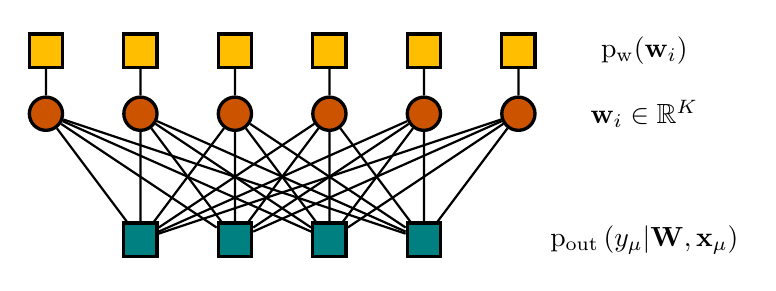
\begin{tikzpicture}[scale=0.8, auto, swap]
			    \foreach \i in {1,...,6}
			        \node[var] (X\i) at (1.5*\i,0) {};
			    \node at (11, 0) {$ \vec{w}_i \in \bbR^K $};
			
			    \foreach \mu in {1,...,4}
			        \node[inter] (Y\mu) at (1.5+1.5*\mu,-2) {};
			    \foreach \i in {1,...,6}
			        \foreach \mu in {1,...,4}
			            \path[edge] (X\i) -- (Y\mu);
			    \node at (10, -2) {};
			    \node (F) at (11, -2) {$ \rp_{\out}\(y_\mu | \mat{W}, \vec{x}_{\mu} \) $};			
			    \foreach \i in {1,...,6} {
			        \node[field] (P\i) at (1.5*\i,1) {};
			        \path[edge] (X\i) -- (P\i);
			    }
			    \node at (11, 1) {$ \rp_\w(\vec{w}_i) $};
			\end{tikzpicture}
			\caption{Factor graph corresponding to the committee machines hypothesis class. The vectorial variables to infer $\vec{w}_i$ are fully connected through the quenched disorder $\vec{y} \sim \rP_{\out^\star} (.)$ and each variable follow a one-body interaction with a separable prior distribution $\rp_\w(\vec{w}_i)$.}
			\label{fig:factor_graph_committee}
			\end{figure}
			
		The partition function at inverse temperature $\beta$ is therefore defined by 
			\begin{align}
			\begin{aligned}
			\mZ_\ndim\(\{\vec{y}, \mat{X}\}; \beta\) &\equiv \rP\(\vec{y},\mat{X}\) = \int_{\bbR^{\ndim\times K}} \d\mat{W} ~ e^{-\beta \mH_\ndim \(\mat{W},\{\vec{y},\mat{X}\}\)}  \\
			&= \int_{\bbR^{\ndim\times K}} \d\vec{w} ~ e^{\beta\( \log \rp_{\out} \(\vec{y} | \mat{W}, \mat{X} \) + \log P_{\w}\(\mat{W}\) \)}\\
			&= \int_{\bbR^{\ndim\times K}} \d\vec{w} ~ \rp_{\out} \(\vec{y} | \mat{W}, \mat{X} \) \rp_{\w}\(\mat{W}\)\,,
			\end{aligned}
			\end{align}
			and can be exactly mapped to Bayesian estimation for $\beta=1$. In the context of \aclink{ERM}, \aclink{MAP} estimation can be analyzed  by taking the limit $\beta\to \infty$.\\
			
			In the considered modern high-dimensional regime with $\ndim \to \infty$, $\nsamples \to\infty$, $\alpha = \nsamples/\ndim = \Theta(1)$ and $K=\Theta(1)$, we are interested in computing the \emph{free entropy} $\Phi$
			\emph{averaged} over the input data $\mat{X}$ and teacher weights $\mat{W}^\star$, or equivalently over the output labels $\vec{y}$ generated from it, defined as
			\begin{align}
				\Phi(\alpha) \equiv \lim_{\ndim \to \infty}  \frac{1}{\ndim}  \EE_{\vec{y},\mat{X}} \[\log  \mZ_\ndim\(\vec{y}, \mat{X}\) \]\,.
				\label{free_entropy}
			\end{align}
			
\begin{remark}
	\begin{itemize}
		\item The distribution $\rP\(\vec{w} | \vec{y}; \mat{X}\)$ is often intractable in the limit $\ndim \to \infty$
		\item Moreover it is still hard to sample efficiently in the high-dimensional regime
	\end{itemize}
\end{remark}

To circumvent this issue:

\begin{itemize}
	\item We can focus only on marginals $\rP(\vec{w}_i; \vec{y}, \mat{X})$ which can been estimated with \textbf{Belief Propagation (BP)} equations and \textbf{Approximate Message Passing (AMP) algorithms}, as illustrated in \Sec\ref{sec:bp_amp}.
	\item We may also try to compute directly the free entropy: we present the replica method in \Sec\ref{sec:replicas} that allows to compute the above average over the random dataset $\{\vec{y}, \mat{X}\}$, that plays the role of the quenched disorder in usual spin glasses. We show the computation for the more involved committee machine model class and generalization of the GLM class, only for \iid data. 
	\item We try to give an idea how these two methods relate and we show they are complementary and consistent.
\end{itemize} 


\begin{remark}
	The cumbersome computation for non \iid data can be performed as well and lead to more complex expressions and has been performed in particular in \cite{kabashima2008inference} in the case of the GLM. 
\end{remark}



					

% replicas %
\newpage

\newpage
\section{Replica computation}
\label{sec:replicas}


\subsection{Heuristic derivation}
	
	In this section, we present the heuristic derivation of the replica formula in the context of  of the \emph{committee machine}. This computation is necessary to properly guess the formula that can then be proven using the adaptive interpolation method.
	 The reader interested in the replica approach to neural networks and the committee machine is invited to look as well to some of the classical papers \cite{gardner1988optimal,mezard1989space,schwarze1992generalization,schwarze1993generalization,schwarze1993learning,monasson1995learning}.\\
	 
	We present here the replica computation of the averaged free entropy $\Phi(\alpha)$ in \eq\eqref{free_entropy} for arbitrary \emph{student} prior and channel distributions $\rP_{\w},\rP_{\w^\star}$ and $\rP_{\out},\rP_{\out^\star}$, so that the computation remains valid for both the Bayes-optimal and mismatched settings.\\
	

	\subsubsection{Replica trick}
	\label{sec:replict_rick}
		The average in eq.~\eqref{free_entropy} is intractable in general, and the computation relies on the so called \emph{replica trick}, that consists in applying the identity  
				\begin{align}
					\EE_{\vec{y},\mat{X}} \[ \lim_{\ndim \to \infty} \frac{1}{\ndim} \log  \mZ_\ndim\(\vec{y}, \mat{X}\) \] =  \lim_{r \to 0} \[ \lim_{\ndim \to \infty}  \frac{1}{\ndim}  \frac{\partial \log \EE_{\vec{y},\mat{X}} \[  \mZ_\ndim\(\vec{y}, \mat{X}\)^r\] }{\partial r} \]\,.
					\label{appendix:replica:committee:replica_trick}
				\end{align}
		The replica trick has been used in a series of previous works to compute the free energy density of GLM for separable distributions \cite{krzakala2012probabilistic} and has been rigorous proven in this case by \cite{barbier2017phase}.\\
		
		Eq.~\eqref{appendix:replica:committee:replica_trick} is interesting in the sense that it reduces the intractable average to the computation of the moments of the averaged partition function, which are easier quantities to compute. Note that for $r \in \bbN$, $\mZ_\ndim\(\vec{y}, \mat{X}\)^r = \prod_{a=1}^r \mZ_\ndim\(\vec{y}, \mat{X}\)$ represents the partition function of $r$ identical non-interacting copies of the initial system, called \emph{replicas}. Taking the quenched average over the disorder will then correlate the replicas, before taking the number of replicas $r\to 0$.	
		Therefore, we assume there exists an analytical continuation so that $r\in \bbR$ and the limit is well defined. Finally, notice that we exchanged the order of the limits $r \to 0$ and $\ndim \to \infty$. These technicalities are crucial points but are not rigorously justified and we will ignore them in the rest of the computation.\\
	
		First, in order to decouple the contributions of the channel $\rP_\out$ and the prior $\rP_\w$, we introduce the variable $\mat{Z} = \frac{1}{\sqrt{\ndim}} \mat{X} \mat{W}$ and a Dirac-delta integral:
			\begin{align}
				\mZ_\ndim\(\vec{y}, \mat{X}\) &= \int_{\bbR^{\nsamples\times K}} \d\vec{z} ~ \rp_{\out}\(\vec{y} | \mat{Z} \) \int_{\bbR^{\ndim\times K}} \d\vec{w} ~ \rp_{\w}\(\mat{W}\) \delta\(\mat{Z} - \frac{1}{\sqrt{\ndim}} \mat{X} \mat{W}\)\,.
			\end{align} 
			Thus the replicated partition function for an integer $r\in \bbN$ in eq.~\eqref{appendix:replica:committee:replica_trick} can be  written as
			\begin{align}
			&\EE_{\vec{y},\mat{X}} \[  \mZ_\ndim\(\vec{y}, \mat{X}\)^r \] \nonumber \\
			&=  \EE_{\vec{y},\mat{X}} \[  \prod_{a=1}^r \int_{\bbR^\nsamples} \d\mat{Z}^a ~ \rp_{\out^a}\(\vec{y} | \mat{Z}^a \) \right. \\
			& \qquad \qquad \left. \times  \int_{\bbR^{\ndim \times K}} \d\mat{W}^a ~ \rp_{\w^a}\(\mat{W}^a\) \delta\(\mat{Z}^a - \frac{1}{\sqrt{\ndim}}\mat{X} \mat{W}^a\)\] \nonumber \\ 
			&= \EE_{\mat{X}} \int_{\bbR^\nsamples} \d \vec{y} ~ \int_{\bbR^{\nsamples \times K}} \d\mat{Z}^\star ~ \rp_{\out^\star}\(\vec{y} | \mat{Z}^\star \)  \\
			& \qquad \qquad \times  \int_{\bbR^{\ndim \times K}} \d\mat{W}^\star ~ \rp_{\w^\star}\(\mat{W}^\star\) \delta\(\mat{Z}^\star - \frac{1}{\sqrt{\ndim}}\mat{X} \mat{W}^\star\)\nonumber \\
			& \times \[  \prod_{a=1}^r \int_{\bbR^{\nsamples \times K}} \d\mat{Z}^a ~ \rp_{\out^a}\(\vec{y} | \mat{Z}^a \) \int_{\bbR^{\ndim\times K}} \d\mat{W}^a ~ \rp_{\w^a}\(\mat{W}^a\) \delta\(\mat{Z}^a - \frac{1}{\sqrt{\ndim}}\mat{X} \mat{W}^a\)\]  \nonumber \\
			&= \int_{\bbR^\nsamples} \d \vec{y} ~ \prod_{a=0}^r \int_{\bbR^{\nsamples \times K}} \d\mat{Z}^a ~ \rp_{\out^a}\(\vec{y} | \mat{Z}^a \) \int_{\bbR^{\ndim \times K}} \d\mat{W}^a ~ \rp_{\w^a}\(\mat{W}^a\) \\
			& \qquad \qquad  \times \underbrace{\EE_{\mat{X}} \prod_{a=0}^r \delta\(\mat{Z}^a - \frac{1}{\sqrt{\ndim}}\mat{X} \mat{W}^a\)}_{(I)}\,. \nonumber
			\end{align}
			Note that the average over $\vec{y}$ is equivalent to the one over the ground truth vector $\mat{W}^\star$ in the case of a \emph{teacher-student}, which can be conveniently grouped with the other terms by just extending the replica indices and
			considering it as a new replica $\mat{W}^0$ with index $a=0$, leading to a total of $r+1$ replicas. 
			
		%%%% Average %%%%
	\subsubsection{Average over the i.i.d input data $\mat{X}$}	
	\label{average_data}	
			Remains to compute the average over $\mat{X}$ in the term $(I)$.
			We suppose that inputs are drawn from an \iid distribution, for example a Gaussian $\rP_{\textrm{x}}(\vec{x}) = \mN_{\vec{x}}\(\vec{0},\mat{I}_\ndim\)$. More precisely, for $(i,j) \in \lb \ndim\rb^2$, $(\mu,\nu) \in \lb \nsamples \rb^2$, $\EE_\mat{X} \[ x_{\mu i} x_{\nu j} \] =  \delta_{\mu\nu} \delta_{ij}$. \\
			By definition, the average in $(I)$ defines the probability density $\rp_{\z^a} (\mat{Z}^a)$ and as $\forall k \in \lb K \rb, \forall \mu \in \lb\nsamples \rb$, $z_{\mu k}^a =\frac{1}{\sqrt{\ndim}} \sum_{i=1}^\ndim x_{\mu i} w_{ik}^a$ is the sum of \iid random variables, the CLT insures that in the thermodynamic limit $\ndim \to \infty$, $z_{\mu k}^a$ follows a Gaussian multivariate distribution, with first moments given by:
			\begin{align}
					\EE_{\mat{X}}[z_{\mu k}^a] &= \frac{1}{\sqrt{\ndim}} \sum_{i=1}^\ndim \EE_{\mat{X}}\[x_{\mu i}\] w_{ik}^a = 0 \spacecase
					\EE_{\mat{X}}[z_{\mu k}^a z_{\nu k'}^b] &= \frac{1}{\ndim} \sum_{ij} \EE_{\mat{X}}\[x_{\mu i} x_{\mu j}\] w_{ik}^a w_{jk'}^b  = \frac{1}{\ndim} \sum_{ij}  \delta_{ij} w_{ik}^a w_{jk'}^b \delta_{\mu \nu} \equiv \delta_{\mu \nu} ~ Q^{a k}_{b k'}. \nonumber
			\end{align}
			
			Notice that averaging over the quenched disorder introduced correlations between replicas, which were initially independent, described by the symmetric \emph{overlap} matrix $\{ Q^{a k}_{b k'}\}_{kk'}$ of size $(r+1)K \times (r+1)K$.
			This matrix order parameter measures the correlations between the replicated matrices $\{\mat{W}^a\}_{a=0}^r$ and is formally defined by
			$$\mat{Q}(\{\mat{W}^a\}_{a=0}^r)\equiv\(\frac{1}{\ndim} \sum_{i=1}^{\ndim} w_{ik}^a w_{ik'}^b \)^{a,b=0..r}_{k,k'=1..K}\,,$$ 
			such that $\forall (a,b) \in \lb 0 : r \rb^2 $, $\mat{Q}^{ab} \in \bbR^{K \times K}$. 
			Therefore, again by the CLT, in the limit $d\to\infty$, the hidden variable $\mat{Z}^a \in \bbR^{\nsamples \times K}$ converges in distribution to the multivariate distribution
			\begin{align}
				\rP_{\z^a}\(\mat{Z}^a|\mat{Q}\) = \exp \left[- \frac{1}{2} \sum_{\mu =1}^\nsamples \sum_{a,b=0}^r \sum_{k,k'=1}^K z^{a}_{\mu k} z^b_{\mu k'}(\mat{Q}^{-1})_{k k'}^{ab} \right] / \( \det{2\pi \mat{Q}} \)^{\frac{\nsamples}{2}}\,.
			\end{align}
				
			Inserting this back in the replicated partition function finally writes
			
			\begin{align}
			&\EE_{\vec{y},\mat{X}} \[  \mZ_\ndim\(\vec{y}, \mat{X}\)^r \] = \nonumber \\
			& \qquad \int_{\bbR^\nsamples} \d \vec{y} ~ \prod_{a=0}^r \int_{\bbR^{\nsamples \times K}} \d\mat{Z}^a ~ \rp_{\out^a}\(\vec{y} | \mat{Z}^a \) \rp_{\z^a}\(\mat{Z}^a|\mat{Q}\) \int_{\bbR^{\ndim \times K}} \d\mat{W}^a ~ \rp_{\w^a}\(\mat{W}^a\)
			\end{align}
						
						
	\subsubsection{Fourier representation}
			Next we introduce the change of variable for the new order parameter $\mat{Q}^{ab}$ with a Dirac-$\delta$ distribution and its Fourier representation. For a variable $x \in \bbR$, the distribution $\delta(x)$ can be written as an integral over a purely imaginary parameter $\hat{x}$:
			\begin{align*}
				\delta\(x\) = \frac{1}{2 i\pi} \int_{i \bbR} \d \hat{x} e^{-\hat{x} x }\,.
			\end{align*}
			
			 Applying the above identity to the change of variable, we obtain
			 \begin{align}
			 \begin{aligned}
			 	&1 = \int_{\bbR^{(K \times r+1)^2 }} \d \mat{Q} \prod_{0 \leq a \leq b \leq r, 1 \leq k,k'\leq K} \delta \(\ndim Q^{ab}_{kk'}-\sum_{i=1}^\ndim w_{ik}^a w_{ik'}^b \)\\
				&\propto \int \int_{\bbR^{(K \times r+1)^2}} \d \mat{Q} \d\hat{\mat{Q}} ~ \exp \( - \ndim \sum_{a=0}^r \sum_{k, k'}^K Q^{aa}_{k k'} \hat{Q}^{aa}_{k k'} - \frac{\ndim}{2} \sum_{a \neq b}^r \sum_{k, k'}^K Q^{a b}_{k k'} \hat{Q}^{a b}_{k k'}  \) \\
				&  \qquad \qquad \times \exp \(\sum_{a=0}^r \sum_{k, k'}^K  \hat{Q}^{a a}_{k k'} w_k^a w_{k'}^a  + \frac{1}{2} \sum_{a \neq b}^r \sum_{k,k'}^K \hat{Q}^{a b}_{k k'} w_k^a w_{k'}^b\) \,,
			\end{aligned}
			\end{align} 
			that involves a new ad-hoc purely imaginary matrix parameter $\hat{\mat{Q}} \in i\bbR^{(K \times (r+1))^2 }$.
			Finally, multiplying the replicated partition function by $1$, using the Cauchy theorem and rotating the integration, it becomes an integral over the symmetric matrices $\mat{Q} \in \bbR^{(K \times r+1)^2}$ and $\hat{\mat{Q}} \in \bbR^{(K \times r+1)^2}$
			 \begin{align*}       
			  &\EE_{\vec{y},\mat{X}} \[  \mZ_\ndim\(\vec{y}, \mat{X}\)^r \] \\
			  &= \int \int_{\bbR^{(K \times r+1)^2}} \d \mat{Q} \d\hat{\mat{Q}} ~ \exp \( - \ndim \sum_{a=0}^r \sum_{k,k'}^K Q^{aa}_{kk'} \hat{Q}^{aa}_{kk'} - \frac{\ndim}{2} \sum_{a \neq b}^r \sum_{k, k'}^K Q^{a b}_{k k'} \hat{Q}^{a b}_{k k'}  \) \\
			  & \qquad \qquad \times \exp \( \sum_{a=0}^r \sum_{k, k'}  \hat{Q}^{a a}_{k k'} w_k^a w_{k'}^a  + \frac{1}{2} \sum_{a \neq b} \sum_{k, k'} \hat{Q}^{a b}_{k k'} w_k^a w_{k'}^b\)\\
			  & \int_{\bbR^\nsamples} \d \vec{y}  \prod_{a=0}^r \int_{\bbR^{\nsamples \times K}} \d\mat{Z}^a ~ \rp_{\out^a}\(\vec{y} | \mat{Z}^a \) \rp_{\z^a}\(\mat{Z}^a | \mat{Q} \) \int_{\bbR^{\ndim \times K}} \d\mat{W}^a ~ \rp_{\w^a}\(\mat{W}^a\) \\
			  &= \int \int_{\bbR^{(K \times r+1)^2}} \d \mat{Q} \d\hat{\mat{Q}} ~ \exp \( - \ndim \sum_{a=0}^r \sum_{k, k'}^K Q^{aa}_{kk'} \hat{Q}^{aa}_{kk'} - \frac{\ndim}{2} \sum_{a \neq b}^r \sum_{k, k'}^K Q^{a b}_{k k'} \hat{Q}^{a b}_{k k'}  \) \\
			  & \qquad \qquad \times \exp \( \sum_{a=0}^r \sum_{k, k'}^K  \hat{Q}^{a a}_{k k'} w_k^a w_{k'}^a  + \frac{1}{2} \sum_{a \neq b}^r \sum_{k,k'}^K \hat{Q}^{a b}_{k k'} w_k^a w_{k'}^b\)\\
			  &  \[\int_\bbR \d y  \prod_{a=0}^r \int_{\bbR^{K}} \d\vec{z}^a ~ \rp_{\out^a}\(y | \vec{z}^a \) \rp_{\z^a}\(\vec{z}^a | \mat{Q} \)\]^\nsamples \[\prod_{a=0}^r \int_{\bbR^{K}} \d\vec{w}^a ~ \rp_{\w^a}\(\vec{w}^a\)\]^{\ndim} \\
			  &\simeq  \int \int_{\bbR^{(K \times r+1)^2}} \d \mat{Q} \d\hat{\mat{Q}} ~ e^{\ndim \Phi^{(r)} (\mat{Q},\hat{\mat{Q}} )} \,,
			\end{align*}    
			where in the last step, we used a Laplace method \cite{Rong89} and omitted the sub-leading factors in the thermodynamic limit $\ndim \to \infty$ to evaluate it as a function of the free entropy potential defined by
			\begin{align}
			\begin{aligned}
				\Phi^{(r)} (\mat{Q},\hat{\mat{Q}}) &\equiv  - \sum_{a=0}^r \sum_{k, k'}^K Q^{a a}_{k k'} \hat{Q}^{a a}_{k k'} -\frac{1}{2}\sum_{a \neq b}^r \sum_{k, k'}^K Q^{a b}_{k k'} \hat{Q}^{a b}_{k k'} \\
				&+ \log \Psi_{\w}^{(r)} (\hat{\mat{Q}})  + \alpha \log \Psi_{\out}^{(r)}(\mat{Q})\,,
			      \spacecase
			      \Psi_{\w}^{(r)} (\hat{\mat{Q}}) &\equiv \displaystyle \prod_{a=0}^r \int_{\bbR^{K}} \d \vec{w}^a ~ 
			      \rp_{\w^a}\(\vec{w}^a\) \\
			      & \hhspace \times \exp \( \sum_{a=0}^r \sum_{k k'}^{K}  \hat{Q}^{a a}_{k k'} w_k^a w_{k'}^a  + \frac{1}{2} \sum_{a \neq b}^r \sum_{k,k'}^{K} \hat{Q}^{a b}_{k k'} w_k^a w_{k'}^b\)\,, \spacecase
			      \Psi_{\out}^{(r)}(\mat{Q}) &\equiv \displaystyle \prod_{a=0}^r  \int_\bbR \d y \int_{\bbR^{K}}  \d \vec{z}^a ~ \rp_{\out^a}\(y | \vec{z}^a\) \rp_{\z^a}\(\vec{z}^a | \mat{Q}\)\,,
			\end{aligned}
			    \label{appendix:intro:replicas:Phi_r}
			\end{align}
			and where we decoupled the variable $\Z^a \in \bbR^{\nsamples \times K}$ and $\mW^a \in \bbR^{\ndim \times K}$ along the rows
			\begin{align*}
				\rp_{\out^a}\(\vec{y} | \mat{Z}^a \) &= \displaystyle \prod_{\mu=1}^\nsamples \rp_{\out^a}\(y_\mu | \vec{z}^a_\mu \)\,, \text{ with } \vec{z}^a_\mu \in \bbR^{K}\,, \\
				\rp_{\z^a} (\mat{Z}^a| \mat{Q}) &= \displaystyle \prod_{\mu=1}^\nsamples \rp(\vec{z}^a_\mu | \mat{Q})\,, \\
				\rp_{\w^a}\(\mat{W}^a\) &= \displaystyle \prod_{i=1}^\ndim \rp_{\w^a}\( \vec{w}^a_i \)\,, \text{ with } \vec{w}^a_i \in \bbR^{K}\,,\\
				\rp_{\z^a}\(\vec{z}^a | \mat{Q}\) &= \exp \left[- \frac{1}{2} \sum_{a,b=0}^r \sum_{k,k'=1}^K z^{a}_{k} z^b_{k'}(\mat{Q}^{-1})_{k k'}^{ab} \right] / \( \det{2\pi \mat{Q}} \)^{\frac{1}{2}}\,.
			\end{align*}
			Note that the averaged replicated partition function of this fully connected model can be expressed as a saddle point equation only because distributions $\rP_{\out},\rP_{\out^\star}$ and $\rP_\w,\rP_{\w^\star}$ are separable so that a pre-factor scaling with the system size $\ndim$ dominates the exponential distribution.
			Finally, switching the two limits $r\to 0$ and $\ndim \to \infty$, the quenched free entropy $\Phi$ simplifies as a saddle point equation
			\begin{equation}
				\Phi (\alpha) = \extr_{ \mat{Q}, \hat{\mat{Q}} } \left\{\lim_{r\rightarrow 0} \frac{\partial \Phi^{(r)}(\mat{Q},\hat{\mat{Q}})}{\partial  r} \right\}\,,
			\end{equation}
			over symmetric matrices $\mat{Q}\in \bbR^{(K \times r+1)^2}$ and $\hat{\mat{Q}} \in \bbR^{(K \times r+1)^2}$.\\
			 
			To summarize, we managed to get rid of the original high-dimensional integrals and replace them by an optimization in the space of matrices, which, in this form, is still intractable. We not only have to search in the space of $(r+1)\times (r+1)$ matrices to find the extremiser of $\Phi^{(r)}$, but we also need to compute the limit $r\to 0^{+}$.
			In the following we will assume a simple Ansatz for these matrices in order to first obtain an analytic expression in $r$ before taking the derivative with respect to $r$.

		\subsection{Replica Symmetric free entropy}
		\label{rs_free_entropy}			
			Our goal is to express the functional $\Phi^{(r)}(\mat{Q},\hat{\mat{Q}})$ appearing in the free entropy as an analytical function of $r$, in order to perform the replica trick. 
			
			\subsubsection{Replica symmetric ansatz}
			To do so, we will assume that the extremum of $\Phi^{(r)}$ is attained at a point in $\mat{Q},\hat{\mat{Q}}$ space such that a \emph{replica symmetry} property is verified. More concretely, we assume: 
			\begin{align}
			\begin{aligned}
			\exists \mat{Q} \in \bbR^{K \times K} \text{ s.t } \quad \forall a \in \lb 0 : r \rb \quad \forall (k,k') \in \lb K \rb^2 \quad Q^{a a}_{k k'} &= Q_{k k'}\,,\\
			\exists \mat{Q}^\star \in \bbR^{K \times K} \text{ s.t } \quad \forall (k,k') \in \lb K \rb^2 \quad Q^{0 0}_{k k'} &= Q^\star_{k k'}\,,\\
			\exists \mat{q} \in \bbR^{K \times K} \text{ s.t } \quad \forall (a < b) \in \lb 0 : r \rb^2 \quad \forall (k,k') \in \lb K \rb^2 \quad Q^{a b}_{k k'} &= q_{k k'}\,,\\
			\exists \mat{m} \in \bbR^{K \times K} \text{ s.t } \quad \forall a \in \lb 0 : r\rb \quad \forall (k,k') \in \lb K \rb^2 \quad Q^{0 a}_{k k'} &= m_{k k'}\,,
			\end{aligned}
			\end{align}
			and similarly for the ad-hoc parameter
			\begin{align}
			\begin{aligned}
			\exists \hat{\mat{Q}} \in \bbR^{K \times K} \text{ s.t } \quad \forall a \in \lb 0 : r \rb \quad \forall (k,k') \in \lb K \rb^2 \quad \hat{Q}^{a a}_{k k'} &= -\frac{1}{2} \hat{Q}_{k k'}\,,\\
			\exists \hat{\mat{Q}}^\star \in \bbR^{K \times K} \text{ s.t } \quad \forall (k,k') \in \lb K \rb^2 \quad \hat{Q}^{0 0}_{k k'} &= \hat{Q}^\star_{k k'}\,, \\
			\exists \hat{\mat{q}} \in \bbR^{K \times K} \text{ s.t } \quad \forall (a < b) \in \lb 0 : r \rb^2 \quad \forall (k,k') \in \lb K \rb^2 \quad \hat{Q}^{a b}_{k k'} &= \hat{q}_{k k'}\,, \\
			\exists \hat{\mat{m}} \in \bbR^{K \times K} \text{ s.t } \quad \forall a \in \lb 0 : r \rb \quad \forall (k,k') \in \lb K \rb^2 \quad \hat{Q}^{0 a}_{k k'} &= \hat{m}_{k k'}\,.
			\end{aligned}\
			\end{align} 
			The factor $-\frac{1}{2}$ is not necessary bu useful to recover commonly used formulations.
			This Ansatz can be represented by symmetric RS matrices $\mat{Q}^{(\rs)} \in \bbR^{(K \times r+1)^2}$ and $\hat{\mat{Q}}^{(\rs)} \in \bbR^{(K \times r+1)^2}$
			\begin{equation}
			\begin{aligned}[c]
			\mat{Q}^{(\rs)} = \scalemath{0.95}{\begin{pmatrix} 
			\mat{Q}^\star & \mat{m} & \cdots & \mat{m} \\
			\mat{m}^\intercal  & \mat{Q}  & \mat{q} & ...  \\
			\vdots & \mat{q} & \ddots & \mat{q}   \\
			\mat{m}^\intercal  &... & \mat{q}  & \mat{Q}     \\
			\end{pmatrix}}
			\end{aligned}
			\hspace{0.2cm}
			\textrm{and} 
			\hspace{0.2cm}
			\begin{aligned}[c]
			\hat{\mat{Q}}^{(\rs)}=\scalemath{0.9}{\begin{pmatrix} 
			 \hat{\mat{Q}}^\star & \hat{\mat{m}} & ... & \hat{\mat{m}}\\
			\hat{\mat{m}}^\intercal &-\frac{1}{2}\hat{\mat{Q}} & \hat{\mat{q}} & ...  \\
			 \vdots & \hat{\mat{q}} & \ddots & \hat{\mat{q}}  \\
			\hat{\mat{m}}^\intercal &... & \hat{\mat{q}} & -\frac{1}{2}\hat{\mat{Q}}\\  
			\end{pmatrix}}\,,
			\end{aligned}
			\end{equation}
			where the \emph{overlap} parameters may be reinterpreted as the scalar product between the replicas
			\begin{align*}
				\forall (a,b) \in \lb r \rb^2,~ \mat{q} = \frac{1}{\ndim} \mat{W}^{a \intercal} \mat{W}^{b}\,,
			\end{align*}
			the self-overlap of each replica
			\begin{align*}
				\forall a \in \lb r \rb,~ \mat{Q} = \frac{1}{\ndim} \mat{W}^{a \intercal} \mat{W}^{a}\,,
			\end{align*}
			the scalar product with the ground truth
			\begin{align*}
				\forall a \in \lb r \rb,~ \vec{m} = \frac{1}{\ndim} \mat{W}^{\star \intercal} \mat{W}^{a}\,,
			\end{align*}
			and the second moment of the ground truth distribution
			\begin{align*}
				\mat{Q}^\star = \frac{1}{\ndim} \mat{W}^{\star \intercal} \mat{W}^{\star}\,.
			\end{align*}
			The above Ansatz simplifies in the scalar GLM case with $K=1$ to
			$q = \frac{1}{\ndim} \vec{w}^a \cdot \vec{w}^b$ for $a \ne b$, a norm $Q= \frac{1}{\ndim} \|\vec{w}^a\|_2^2$, an overlap with the ground truth $m =\frac{1}{\ndim} \vec{w}^a \cdot \vec{w}^\star$ and a second moment $Q^\star= \frac{1}{\ndim} \|\vec{w}^\star\|_2^2$.\\
		
		\subsubsection{Decomposition of the free entropy functional}
			Let's compute separately the terms involved in the functional $\Phi^{(r)}(\mat{Q},\hat{\mat{Q}})$ in \eqref{appendix:intro:replicas:Phi_r} by applying this Ansatz: the first is a trace term, the second term $\Psi_{\w}^{(r)}$ depends on the prior distributions $\rP_\w$, $\rP_{\w^\star}$ and finally the third term $\Psi_{\out}^{(r)}$ depends on the channel distributions $\rP_{\out^\star}$, $\rP_\out$.
						
		\paragraph{Trace term} 
				The trace term in \eqref{appendix:intro:replicas:Phi_r} can be easily computed at the RS fixed point and takes the following form
				\begin{align}
				\begin{aligned}
					&\left. - \sum_{a=0}^r \sum_{k, k'}^K Q^{a a}_{k k'} \hat{Q}^{a a}_{k k'} -\frac{1}{2}\sum_{a \neq b}^r \sum_{k, k'}^K Q^{a b}_{k k'} \hat{Q}^{a b}_{k k'} \right|_{\rs} \\
					&= - \tr{\mat{Q}^\star \hat{\mat{Q}}^\star} + \frac{1}{2} r \tr{\mat{Q} \hat{\mat{Q}}} -  r \tr{\mat{m} \hat{\mat{m}}}  - \frac{r(r-1)}{2} \tr{\mat{q} \hat{\mat{q}}}\,,
				\end{aligned}
				\end{align}
				and taking the derivative and the limit $r\to 0$ we obtain
				\begin{align}
				\begin{aligned}
					&\lim_{r \to 0} \partial_r \( \left. - \sum_{a=0}^r \sum_{k, k'}^K Q^{a a}_{k k'} \hat{Q}^{a a}_{k k'} -\frac{1}{2}\sum_{a \neq b}^r \sum_{k, k'}^K Q^{a b}_{k k'} \hat{Q}^{a b}_{k k'} \)\right|_{\rs} \\
					&  \qquad \qquad = \frac{1}{2} \tr{\mat{Q} \hat{\mat{Q}}} -  \tr{\mat{m} \hat{\mat{m}}}  + \frac{1}{2} \tr{\mat{q} \hat{\mat{q}}}
					\label{appendix:replicas:committee:trace} 
				\end{aligned}
				\end{align}
			
			\paragraph{Prior integral $\Psi_{\w}^{(r)}$} Evaluated at the RS fixed point the quadratic form reads			      
				\begin{align*}
					&\sum_{a=0}^r \sum_{k k'}  \hat{Q}^{a a}_{k k'} w_k^a w_{k'}^a  + \frac{1}{2} \sum_{a \neq b} \sum_{k,k'} \hat{Q}^{a b}_{k k'} w_k^a w_{k'}^b\\
					&= \vec{w}^{\star \intercal} \hat{\mat{Q}}^\star \vec{w}^{\star} + \sum_{a=1}^r \vec{w}^{\star \intercal} \hat{\mat{m}} \vec{w}^a - \frac{1}{2} \sum_{a=1}^r  \vec{w}^{a \intercal} \hat{\mat{Q}} \vec{w}^{a} + \frac{1}{2} \sum_{1 \leq a \ne b \leq r}  \vec{w}^{a \intercal} \hat{\mat{q}} \vec{w}^{b} \\
					&= \vec{w}^{\star \intercal} \hat{\mat{Q}}^\star \vec{w}^{\star} + \sum_{a=1}^r \vec{w}^{\star \intercal} \hat{\mat{m}} \vec{w}^a - \frac{1}{2} \sum_{a=1}^r  \vec{w}^{a \intercal} \(\hat{\mat{Q}} + \hat{\mat{q}} \) \vec{w}^{a} + \frac{1}{2} \(\sum_{a=1}^r  \vec{w}^{a} \)^\intercal \hat{\mat{q}} \(\sum_{a=1}^r  \vec{w}^{a} \)\,.
				\end{align*}
				
				Using a Hubbard-Stratonovich transformation:
				\begin{proposition}[Hubbard-Stratonovich transformation]
				\label{prop:hubbard}
					 For $\bxi \sim \mN\(\vec{0},\rI_\ndim\)$ and a symmetric positive definite matrix $\mat{A} \in \bbR^{\ndim \times \ndim}$, for all $\vec{x} \in \bbR^{\ndim}$
					 \begin{align}
					\EE_{\bxi}\exp\(  \bxi^\intercal \mat{A}^{1/2} \vec{x} \) = \(2\pi\)^{-\ndim/2} \int_{\bbR^\ndim} \d \bxi e^{-\frac{1}{2} \vec{x}^\intercal \vec{x} + \bxi^\intercal \mat{A}^{1/2} \vec{x} } = e^{\frac{1}{2} \vec{x}^\intercal \mat{A} \vec{x} }\,,
					\end{align}
				\end{proposition}
				
				the prior integral can be further simplified 
				
				\begin{align}
				\begin{aligned}
					&\left.\Psi_{\w}^{(r)} (\hat{\mat{Q}})\right|_{\rs} = \displaystyle \int_{\bbR^{(r+1) \times K}} \d \mat{W} ~ 
			        \rp_{\w}\(\mat{W}\) e^{\sum_{a=0}^r \sum_{k, k'} ^K \hat{Q}^{a a}_{k k'} w_k^a w_{k'}^a  + \frac{1}{2} \sum_{a \neq b} \sum_{k,k'}^K \hat{Q}^{a b}_{k k'} w_k^a w_{k'}^b} \\
					&= \EE_{\bxi, \vec{w}^\star \sim \rP_{\w^\star}} \[ e^{\vec{w}^{\star \intercal} \hat{\mat{Q}}^\star \vec{w}^{\star} } \EE_{\vec{w} \sim \rP_{\w}} \[ e^{\( \vec{w}^\intercal \hat{\vec{m}} \vec{w}^\star  - \frac{1}{2}\vec{w}^\intercal  (\hat{\mat{Q}} + \hat{\mat{q}}) \vec{w} + \vec{w}^\intercal \hat{\mat{q}}^{1/2} \bxi \) } \]^r   \]\,.
				\end{aligned}
				\label{appendix:replicas:committee:Psi_w_rs}
				\end{align}
				
			\paragraph{Detailed computation of $\(\mat{Q}^{(\rs)}\)^{-1}$}
				Let us focus on the matrix $\mat{Q}^{(\rs)}$ involved in the expression of $\Psi_{\out}^{(r)}$ in \eqref{appendix:intro:replicas:Phi_r}.
				Given the replica symmetric ansatz, we must compute the determinant and inverse matrix of the matrix $\bSigma \equiv \mat{Q}^{(\rs)}$.
				
				We use tensor products notations $\otimes$ for matrices living in $\bbR^{ r \times r } \otimes  \bbR^{ K \times K }$. Let us recall some basic properties of the tensor product of two matrices $\mat{A} \in \bbR^{r \times r}$ and $\mat{B} \in \bbR^{K \times K}$:
			\begin{align}
				(\mat{A} \otimes \mat{B})^{-1} &= \mat{A}^{-1} \otimes \mat{B}^{-1} \\
				\det{\mat{A} \otimes \mat{B}} &= \det{\mat{A}}^K \det{\mat{B}}^r \\
				\forall \mat{C}, \mat{D} \quad (\mat{C} \otimes \mat{D}) (\mat{A} \otimes \mat{B}) &= (\mat{C} \mat{A}) \otimes (\mat{D} \mat{B}) \\
				\text{Sp}(\mat{A} \otimes \mat{B}) &= \{\lambda_i \mu_j \quad  / \lambda_i \in \text{Sp}(\mat{A}),\mu_j\in \text{Sp}(\mat{B}) \}
			\end{align}
			
			Next we denote the \emph{reduced} matrix 
			\begin{align}
				\bSigma_r \equiv \begin{pmatrix}
				 \mat{Q} & \mat{q} & \cdots & \mat{q} \\
				 \mat{q} & \mat{Q} & \cdots & \mat{q} \\
				 \vdots & \vdots & \ddots & \vdots \\
				 \mat{q} & \mat{q} & \cdots & \mat{Q} \\
				\end{pmatrix} =  \mat{I}_r \otimes (\mat{Q} - \mat{q}) + \mat{J}_r \otimes \mat{q}\,,
			\end{align}
			where $\mat{J}_r$ is the rank-1 matrix with all elements equal to 1. Finally, some basic linear algebra formulas allow us to reduce the problem of computing $\det{\bSigma}$ and $\bSigma^{-1}$ to those of $\bSigma_r$. 
			
		\paragraph{Calculation of $\mat{S}$} 
			We define the $K \times K$ matrix :
			\begin{align}
				\mat{S} \equiv \mat{Q}^\star - (\vec{1}_r^\intercal
				\otimes \mat{m}) \bSigma_r^{-1} (\vec{1}_r
				\otimes \mat{m}^\intercal)  
			\end{align}
			
			Let us compute $\mat{S}$: 
			\begin{align}
				\begin{aligned}
				\mat{S} &\equiv \mat{Q}^\star - (\vec{1}_r^\intercal
				\otimes \mat{m}) \bSigma_r^{-1} (\vec{1}_r
				\otimes \mat{m}^\intercal)   \nonumber \\
				&= \mat{Q}^\star - r \mat{m} (\mat{Q} - \mat{q})^{-1} \mat{m}^\intercal + r^2 \mat{m} (\mat{Q} + (r-1)\mat{q})^{-1} \mat{q} (\mat{Q} - \mat{q})^{-1} \mat{m}^\intercal \nonumber \\
				&= \mat{Q}^\star - r \mat{m}  \(\mat{I}_K - n (\mat{Q} + (r-1)\mat{q})^{-1}  \mat{q} \)(\mat{Q} - \mat{q})^{-1} \mat{m}^\intercal \nonumber \\
				&= \mat{Q}^\star - r \mat{m} (\mat{Q} + (r-1)\mat{q})^{-1} \(\mat{Q} + (r-1)\mat{q} - r  \mat{q} \) (\mat{Q} - \mat{q})^{-1} \mat{m}^\intercal \nonumber \\
				&= \mat{Q}^\star - r \mat{m} (\mat{Q} + (r-1)\mat{q})^{-1} \mat{m}^\intercal
				\end{aligned}
			\end{align}
				
		\paragraph{Calculation of $\bSigma_r^{-1}$}
			
			$\bSigma_r$ can be easily analyzed, thanks to a slight generalization of the Sherman-Morrison formula.
			\begin{align}
				\bSigma_r =  \mat{I}_r \otimes (\mat{Q} - \mat{q}) + \mat{J}_r \otimes \mat{q} =  \mat{I}_r \otimes (\mat{Q} - \mat{q}) + \vec{1}_r \vec{1}_r^\intercal \otimes  \bq
			\end{align}
			So that the determinant reads
			\begin{align}
				\det{\bSigma_r} &= \det{\mat{Q} - \mat{q}}^r \det{\mat{I}_K + ( \vec{1}^\intercal \otimes \mat{q}) (\mat{I}_r \otimes (\mat{Q} - \mat{q}))^{-1} (\vec{1} \otimes \mat{I}_K)} \nonumber \\
				&= \det{\mat{Q} - \mat{q}}^r \det{ \mat{I}_K + r \bq (\mat{Q} - \mat{q})^{-1} } \nonumber \\
				\det{\bSigma_r} &=  \det{\mat{Q} - \mat{q}}^{r-1} \det{\mat{Q} + (r-1)\mat{q} }\,,
			\end{align}
			
			and the inverse 
			\begin{align}
			\bSigma_r^{-1} &= \mat{I}_r \otimes (\mat{Q} - \mat{q})^{-1} \\
			& - \(\mat{I}_r \otimes (\mat{Q} - \mat{q})^{-1}\) \( \vec{1}_r \otimes \mat{I}_K \) \( \mat{I}_K + r \mat{q} (\mat{Q} - \mat{q})^{-1}\)^{-1} \( \vec{1}_r^\intercal \otimes \mat{q} \) \(\mat{I}_r \otimes (\mat{Q} - \mat{q})^{-1}\) \nonumber \\
			&=  \mat{I}_r \otimes (\mat{Q} - \mat{q})^{-1} - \mat{J}_r \otimes \((\mat{Q} + (r-1)\mat{q})^{-1} \mat{q} (\mat{Q} - \mat{q})^{-1}\)
			\end{align}
			
		
		\paragraph{Determinant of $\mat{Q}^{(\rs)}$}
			Therefore we obtain:
			\begin{align}
				\begin{aligned}
				\det{\bSigma} &= \det{\mat{Q}^{(\rs)}}=  \det{\bSigma_r} \det{\mat{S}}\\
					&=\det{\mat{Q} - \mat{q}}^{r-1} \det{\bQ + (r-1)\mat{q}} \det{\mat{Q}^\star - r \mat{m} (\mat{Q} + (r-1)\mat{q})^{-1} \mat{m}^\intercal}
				\end{aligned}
				\label{det_rs}
			\end{align}
		
		\paragraph{Inverse of $\mat{Q}^{(\rs)}$}
			The inverse of the block matrix reads:
			\begin{align*}
				\bSigma^{-1} &= \begin{pmatrix}
					\mat{S}^{-1} & - \mat{S}^{-1} (\vec{1}_r^\intercal
					\otimes \mat{m})  \bSigma_r^{-1} \\
					- \bSigma_r^{-1} (\vec{1}_r
					\otimes \mat{m}^\intercal)   \mat{S}^{-1} & \bSigma_{r}^{-1} + \bSigma_{r}^{-1} (\vec{1}_r
					\otimes \mat{m}^\intercal) \mat{S}^{-1} (\vec{1}_r^\intercal
					\otimes \mat{m}) \bSigma_{r}^{-1}
					\end{pmatrix} 
			\end{align*}
			
			where each block can be computed separately. The top diagonal simply reads
			\begin{align*}
				\mat{S} ^{-1} &= \(\mat{Q}^\star - r \mat{m} (\mat{Q} + (r-1)\mat{q})^{-1} \mat{m}^\intercal\)^{-1}
			\end{align*}		
			and the off-diagonal blocks read:
			\begin{align}
			& - \bSigma_r^{-1} (\vec{1}_r
			\otimes \mat{m}^\intercal)  \mat{S}^{-1} =\\
			&\quad - \vec{1} \otimes \(\mat{Q} + (r-1)\mat{q})^{-1} \mat{m}^\intercal\(\mat{Q}^\star - r \mat{m} (\mat{Q} + (r-1)\mat{q})^{-1} \mat{m}^\intercal\)^{-1} \) \nonumber \\
			& - \mat{S}^{-1} (\vec{1}_r^\intercal
			\otimes \mat{m})  \bSigma_r^{-1} =\\
			& \quad  - \vec{1}_r^\intercal
			\otimes \(\(\mat{Q}^\star - r \mat{m} (\mat{Q} + (r-1)\mat{q})^{-1} \mat{m}^\intercal\)^{-1}  \mat{m} (\mat{Q} + (r-1)\mat{q})^{-1} \)]  \nonumber
			\end{align}
			
			The bottom diagonal block is a bit more involved : 
			\begin{align}
				\bSigma_{r}^{-1} &+ \bSigma_{r}^{-1} (\vec{1}_r
				\otimes \mat{m}^\intercal) \mat{S}^{-1} ( \vec{1}_r^\intercal
				\otimes \mat{m}) \bSigma_{r}^{-1} \nonumber \\
				&= \mat{I}_r \otimes (\mat{Q} - \mat{q})^{-1} - \mat{J}_r \otimes \mat{A}
			\end{align}
			with 
			\begin{align}
				\mat{A} &\equiv (\mat{Q} + (r-1)\mat{q})^{-1} \mat{q} (\mat{Q} - \mat{q})^{-1} \\
				& - (\mat{Q} + (r-1)\mat{q})^{-1} \mat{m}^\intercal\(\mat{Q}^\star - r \mat{m} (\mat{Q} + (r-1)\mat{q})^{-1} \mat{m}^\intercal\)^{-1}\mat{m} (\mat{Q} + (r-1)\mat{q})^{-1}	\nonumber
			\end{align}

			Finally we observe that $\bSigma^{-1}$ is also a block matrix of the form 
			\begin{equation}
				   \bSigma^{-1} = \(\mat{Q}^{(\rs)}\)^{-1}=\begin{bmatrix}
				   \td{\mat{Q}}^\star & \td{\mat{m}} & \cdots & \td{\mat{m}}  \\
				   \td{\mat{m}}^\intercal & \td{\mat{Q}} & \td{\mat{q}} & \cdots \\
				   \vdots & \td{\mat{q}} & \ddots & \td{\mat{q}} \\
				   \td{\mat{m}}^\intercal & \cdots & \td{\mat{q}} & \td{\mat{Q}} \\
				  \end{bmatrix}
			\end{equation}
			with 
			\begin{align*}
				&\td{\mat{Q}}^\star = \(\mat{Q}^\star - r \mat{m} (\mat{Q} + (r-1) \mat{q})^{-1} \mat{m}^\intercal \)^{-1}   \spacecase
				&\td{\mat{m}} = -\(\mat{Q}^\star - r \mat{m} (\mat{Q} + (r-1) \mat{q})^{-1} \mat{m}^\intercal \)^{-1} \mat{m} ( \mat{Q} + (r-1) \mat{q})^{-1}  \spacecase
				&\td{\mat{Q}} = (\mat{Q}-\mat{q})^{-1} - (\mat{Q} +(r-1) \mat{q})^{-1} \mat{q} (\mat{Q}-\mat{q})^{-1} \\
				& \qquad  + ( \mat{Q} + (r-1) \mat{q} )^{-1} \mat{m}^\intercal \\ 
				& \qquad \qquad \times \(\mat{Q}^\star - r \mat{m} ( \mat{Q} + (r-1) \mat{q})^{-1} \mat{m}^\intercal \)^{-1} \mat{m} ( \mat{Q} + (r-1)\mat{q})^{-1}\spacecase
				&\td{\mat{q}} = \td{\mat{Q}} - (\mat{Q}-\mat{q})^{-1}
			\end{align*}
									
			\paragraph{Channel integral $\Psi_{\out}^{(r)}$}
				The quadratic form in $\rp_{\z^a}(\mat{z}^a | \mat{Q}^{(\rs)}$ reads				
				\begin{align*}
					&- \frac{1}{2} \sum_{a,b} \sum_{k,k'} z^{a}_{k} z^b_{k'}(\mat{Q}^{-1})_{k k'}^{ab} \\
					&= -\frac{1}{2} \vec{z}^{\star \intercal} \td{\mat{Q}}^\star \vec{z} 
					-\sum\limits_{a=1}^{r} \vec{z}^{\star \intercal} \td{\mat{m}} \vec{z}^{a}\\
					&
					\qquad \qquad  -\frac{1}{2}\sum\limits_{a=1}^{r} \vec{z}^{a \intercal} \( \td{\mat{Q}} - \td{\mat{q}} \) \vec{z}^{a}
					-\frac{1}{2} \(\sum\limits_{a}^{r} \vec{z}^{a}\)^\intercal \td{\mat{q}} \(\sum\limits_{a}^{r} \vec{z}^{a}\) \,,
				\end{align*}
				and using another Gaussian transformation, see Prop.~\ref{prop:hubbard}, we finally obtain
				\begin{align}
				&\left. \Psi_{\out}^{(r)}(\mat{Q}) \right|_{\rs} =  \displaystyle \int \d y \int_{\bbR^{(r+1) \times K}}  \d \mat{Z} ~ 
			      \rp_{\out}\(y | \mat{Z}\) \rp\(\mat{Z} | \mat{Q}\) \nonumber \\
			      &= \displaystyle \int \d y \int_{\bbR^{(r+1) \times K}}  \d \mat{Z} 
			      \rp_{\out}\(y | \mat{Z}\) e^{- \frac{1}{2} \sum_{a,b=0}^r \sum_{k,k'=1}^K z^{a}_{k} z^b_{k'}(\mat{Q}^{-1})_{k k'}^{ab} } / \( \det{2\pi \mat{Q}}^{(\rs)} \)^{\frac{1}{2}}
				\nonumber \\
				&= \int \d y ~ \EE_{\bxi} \e^{- \frac{1}{2}\log(\det{2\pi \mat{Q}^{(\rs)}} )} \times \int \d \vec{z}^\star ~ \rp_{\out^\star}\(y | \vec{z}^\star \) e^{ -\frac{1}{2} \vec{z}^{\star \intercal} \td{\mat{Q}}^\star \vec{z}^\star} \label{Psi_out_rs} \\ 
				& \times\[ \int \d \vec{z} ~ \rp_{\out}\(y | \vec{z}\) \exp\( - \vec{z}^{\star \intercal} \td{\mat{m}} \vec{z} - \frac{1}{2} \vec{z}^\intercal \( \td{\mat{Q}} - \td{\mat{q}} \) \vec{z}  + \vec{z}^\intercal (-\td{\mat{q}})^{1/2} \bxi\) \]^r\,, \nonumber
				\end{align}
				with $\det{\mat{Q}^{(\rs)}}$ given by \eqref{det_rs}.
			
		\subsubsection{Consistency conditions $r\to 0$: $\Theta(1)$ terms}
			It remains to take the limit $r \to 0^+$ of the expressions for $\Psi_{\w}^{(r)}$ and $\Psi_{\out}^{(r)}$ that are now analytical in $r$.
			%
			First, our assumptions must be consistent and thus we need to check the consistency conditions in the limit $r \to 0$. Indeed, if $\Phi^{(r)}$ is finite we could obtain divergence taking the limit $\lim_{r \to 0} \frac{1}{r} \Phi^{(r)} = \infty$. Therefore to avoid such divergence, we must at least impose that $\lim_{r \to 0} \Phi^{(r)} = 0$:			  
			\begin{align*}
				\lim_{r\to 0} \Phi^{(r)} (\mat{Q},\hat{\mat{Q}}) &= - \tr{\mat{Q}^\star \hat{\mat{Q}}^\star} +\log \Psi_{\w}^{0} (\hat{\mat{Q}}^\star)+\alpha \log \Psi_{\out}^{0}(\mat{Q}^\star)
			\end{align*}	
			with 
			\begin{align*}
				\Psi_{\w}^{0} (\hat{\mat{Q}}^\star) &\equiv \EE_{\vec{w}^\star} \exp\( \vec{w}^{\star \intercal}  \hat{\mat{Q}}^\star \vec{w}^{\star}\)\,, \spacecase 
				\Psi_{\out}^{0}(\mat{Q}^\star) &\equiv \int_\bbR \d y ~  \int \d \vec{z}^\star ~ \rp_{\out^\star}\(y | \vec{z}^\star \) \mN_{\vec{z}^\star}\(\vec{0}, \mat{Q}^\star \)  = 1 \,.
			\end{align*}		
			Taking the saddle point equations over $\mat{Q}^\star$ and $\hat{\mat{Q}}^\star$, imposing the consistency condition $\lim_{r\to 0} \Phi^{(r)} (\mat{Q},\hat{\mat{Q}}) = 0$, we finally obtain
			\begin{align}
				\hat{\mat{Q}}^\star = \mat{0} \andcase \mat{Q}^\star = \EE_{\vec{w}^\star}\[ \vec{w}^{\star \intercal} \vec{w}^{\star} \]\,.
				\label{appendix:replicas:committee:consistency}
			\end{align}
			
		\subsubsection{Replica trick $r \to 0$ limit: $\Theta(r)$ terms}
			Imposing the conditions \eqref{appendix:replicas:committee:consistency} avoids divergence in the replica trick, and we can therefore proceed with the $\Theta(r)$ terms.  
				
		\paragraph{Prior integral $\Psi_{\w}^{(r)}$}
			The limit $r\to 0$ and the derivative of the logarithm of the prior integral \eqref{appendix:replicas:committee:Psi_w_rs} can be trivially computed
			\begin{align*}
			&\lim_{r \to 0} \partial_r \left. \log \Psi_{\w}^{(r)} (\hat{\mat{Q}})\right|_{\rs} \\
			&= \EE_{\bxi, \vec{w}^\star} \\
			& \times \log \[ \EE_{\vec{w}}  \exp \(\[  \vec{w}^{\star \intercal} \hat{\mat{m}} \vec{w} - \frac{1}{2} \vec{w}^\intercal (\hat{\mat{Q}} + \hat{\mat{q}}) \vec{w} + \bxi^\intercal \hat{\mat{q}}^{1/2}  \vec{w} \] \) \]\,,
			\end{align*}	
			with $\bxi \sim \mN(\vec{0},\mat{I}_K)$ and $\vec{w}^\star \sim \rP_{\w^\star}$. 
			To conclude, we can symmetrize and decouple the \emph{teacher} and \emph{student} expectations $\EE_{\vec{w}^\star},\EE_{\vec{w}}$. By performing the change of variable $\bxi \leftarrow \bxi + \hat{\mat{q}}^{-1/2} \hat{\mat{m}} \vec{w}^\star$. We finally obtain		
			\begin{align}
			&\lim_{r \to 0} \partial_r \left. \log \Psi_{\w}^{(r)} (\hat{\mat{Q}})\right|_{\rs} \nonumber \\ 
			&=  \EE_{\bxi, \vec{w}^\star}\exp\(-\frac{1}{2} \vec{w}^{\star \intercal} \hat{\mat{m}}^\intercal \hat{\mat{q}}^{-1}\hat{\mat{m}} \vec{w}^\star + \bxi^\intercal \hat{\mat{q}}^{-1/2} \hat{\mat{m}} \vec{w}^\star  \)  \label{appendix:replicas:committee:log_Psi_w} \\
			& \hspace{1cm} \times \log \[ \EE_{\vec{w}}  \exp \(\[ - \frac{1}{2}\vec{w}^{\intercal} (\hat{\mat{Q}} + \hat{\mat{q}})\vec{w}  + \bxi^\intercal \hat{\mat{q}}^{1/2} \vec{w} \] \) \] \nonumber \\
			&\equiv \EE_{\bxi, \vec{w}^\star} \mZ_{\w^\star}\(\hat{\mat{m}}\hat{\mat{q}}^{-1/2} \bxi, \hat{\mat{m}}^\intercal \hat{\mat{q}}^{-1}\hat{\mat{m}} \) \log \mZ_\w\(\hat{\mat{q}}^{1/2} \bxi , \hat{\mat{Q}} + \hat{\mat{q}}\)\,, \nonumber
			\end{align}
			with the corresponding denoising distribution $\rQ_\w$ and functions $\mZ_{\w^\star},\mZ_{\w}$ defined by
		\begin{align}
			\begin{aligned}
			\rQ_{\w}(\vec{w}; \bgamma, \bLambda) & \equiv \displaystyle \frac{\rP_{\w}(\vec{w}) }{\mZ_{\w} (\bgamma,\bLambda)} e^{ - \frac{1}{2} \vec{w}^\intercal \bLambda \vec{w}  + \bgamma^\intercal \vec{w}  }\,, \\
			\mZ_{\w} (\bgamma,\bLambda) &\equiv \EE_{\vec{w}\sim \rP_\w} \[ e^{ - \frac{1}{2} \vec{w}^\intercal \bLambda \vec{w}  + \bgamma^\intercal \vec{w}  } \] = \int_{\bbR^K} \d \vec{w} ~ \rp_{\w}(\vec{w})  e^{ - \frac{1}{2} \vec{w}^\intercal \bLambda \vec{w}  + \bgamma^\intercal \vec{w}  }\,,
			\end{aligned}
		\label{distributions:committee_prior}
		\end{align}
		respectively with distribution $\rP_{\w^\star}$ and $\rP_\w$.

		\paragraph{Prior integral $\Psi_{\out}^{(r)}$}
			The limit $r\to 0$ and the derivative of the logarithm of the channel integral \eqref{Psi_out_rs} is more tricky. First, the limit of the determinant \eqref{det_rs} simplifies easily and yields
			\begin{align*}
				\det{\mat{Q}^{(\rs)}} \underlim{r}{0} \det{\mat{Q}^\star}
			\end{align*}
			and the matrix elements of $\(\mat{Q}^{(\rs)}\)^{-1}$ in this limit become
			\begin{align*}
				\td{\mat{Q}}^\star & \underlim{r}{0} \(\mat{Q}^\star\)^{-1}\,,  \spacecase
				\td{\mat{m}} & \underlim{r}{0} -\(\mat{Q}^\star \)^{-1} \mat{m} ( \mat{Q} - \mat{q})^{-1}\,,  \spacecase
				\td{\mat{q}} & \underlim{r}{0} - (\mat{Q} - \mat{q})^{-1}\(\mat{q} -  \mat{m}^\intercal \(\mat{Q}^\star \)^{-1} \mat{m} \)( \mat{Q}-\mat{q})^{-1}\,, \spacecase
				\td{\mat{Q}} & \underlim{r}{0}  \td{\mat{q}} + (\mat{Q}-\mat{q})^{-1}\,.
			\end{align*}
			
			To take properly the $r\to 0$ limit, let us first perform the change of variable $\bxi \leftarrow \bxi - (-\td{\mat{q}})^{1/2} \td{\mat{m}}^\intercal \vec{z}^\star $ in \eqref{Psi_out_rs} so that 
			\begin{align}
			\begin{aligned}
			\left. \Psi_{\out}^{(r)}(\mat{Q}) \right|_{\rs} &= \displaystyle  \int_\bbR \d y \EE_{\bxi} J_0 (y, \bxi, r) \times J_1(y, \bxi, r)^r \\
			J_0 (y, \bxi, r) &=  \e^{- \frac{1}{2}\log(\det{2\pi \mat{Q}^{(\rs)}} )} \\
			& \times \int_{\bbR^K} \d \vec{z}^\star \rp_{\out^\star} ~ \(y | \vec{z}^\star \) e^{ -\frac{1}{2} \vec{z}^{\star \intercal} \(\td{\mat{Q}}^\star - \td{\mat{m}}^\intercal \td{\mat{q}}^{-1} \td{\mat{m}} \) \vec{z}^\star + \bxi^\intercal (-\td{\mat{q}})^{1/2} \td{\mat{m}}^\intercal \vec{z}^{\star}   } \\
			J_1(y, \bxi, r) &= \int_{\bbR^K} \d \vec{z}  ~ \rp_{\out}\(y | \vec{z}\) e^{-\frac{1}{2}  \vec{z}^\intercal \( \td{\mat{Q}} - \td{\mat{q}} \) \vec{z}  + \vec{z}^\intercal (-\td{\mat{q}})^{1/2} \bxi }
			\end{aligned}
			\end{align}	
			so that the integral may be written as follows:
			\begin{align*}
				&\log\(\Psi_{\out}^{(r)}\) = \log \int \d y \EE_{\bxi} J_0(y,\bxi, r) J_1(y,\bxi, r)^r\\
				&=  \log \int_\bbR \d y  \EE_{\bxi} \[ J_0(y, \bxi, 0) + r \partial_r J_0(y, \bxi, 0) + r J_0(y, \bxi, 0) \log J_1(y, \bxi, 0) + \Theta(r^2) \]\\
				&= \log \(1 + r \int_\bbR \d y \times \EE_{\bxi} \[ \partial_r J_0(y, \bxi, 0) + J_0(y, \bxi, 0) \log J_1(y, \bxi, 0) + \Theta(r^2)  \]  \)\\
				&=  r \int_\bbR \d y \times \EE_{\bxi} \[ \partial_r J_0(y, \bxi, 0) + J_0(y, \bxi, 0) \log J_1(y, \bxi, 0)  \] + \Theta(r^2) 
			\end{align*}

	where we used the consistency condition $\int_\bbR \d y \times \EE_{\bxi} J_0(y, \bxi, 0)=1$. The first term can be evaluated similarly
		\begin{align*}
			&\int_\bbR \d y \times \EE_{\bxi} \partial_r J_0(y, \bxi, 0) = \partial_r \[ \int_\bbR \d y \times \EE_{\bxi} J_0(y, \bxi, r) \]_{r=0} \\
			&=  \partial_r \[  \e^{- \frac{1}{2}\log(\det{2\pi \mat{Q}^{(\rs)}} )} \int_{\bbR^K} \d \vec{z}^\star e^{ -\frac{1}{2} \vec{z}^{\star \intercal} \(\td{\mat{Q}}^\star \) \vec{z}^\star}  \]_{r=0} \\
			&= \partial_r \[  \e^{- \frac{1}{2}\log(\det{ \td{\mat{Q}}^\star}  \det{\mat{Q}^{(\rs)}} )} \]_{r=0} = ... = 0 	
			\end{align*}

		Finally we obtain:
			\begin{align*}
			    &\lim\limits_{r\to 0} \partial_r \log\(\Psi_{\out}^{(r)}\) = \int_\bbR \d y \EE_{\bxi}  J_0 (y,\bxi) \log J_1 (y,\bxi) = \lim_{r\to 0} \int_\bbR \d y \EE_{\bxi}  J_0 (y,\bxi) J_1 (y,\bxi)^r
			\end{align*}
			with
			\begin{align*}
			    &J_{0}(y,\bxi) \equiv \e^{- \frac{1}{2}\log(\det{2\pi \mat{Q}^\star} )} \int_{\bbR^K} \d \vec{z}^\star \rp_{\out^\star}\left(y|\vec{z}^\star \right) e^{-\frac{1}{2} \vec{z}^{\star \intercal} \mat{N} \vec{z}^{\star} + \bxi^\intercal \mat{M} \vec{z}^{\star}   }\\
			    &J_{1}(y,\bxi) \equiv \int_{\bbR^K} \d \vec{z} ~\rp_{\out}\(y|\vec{z}\)e^{-\frac{1}{2} \vec{z}^\intercal \(\mat{Q}- \mat{q}\)^{-1} \vec{z} + \vec{z}^\intercal \mat{P} \bxi } \\
			    &= \EE_{\vec{z}\sim\mN\(\vec{0}, \mat{I}_K\)} ~\rp_{\out}\(y|\(\mat{Q}-\mat{q}\)^{1/2} \vec{z}\)e^{\bxi^\intercal \mat{P} \(\mat{Q}-\mat{q}\)^{1/2} \vec{z} }
			\end{align*}
			where we changed the variable $\vec{z} \leftarrow \(\mat{Q}-\mat{q}\)^{-1/2} \vec{z}$ and used the fact that with the second formulation the determinant term at the power $r$ goes away in the limit $r\to 0$ and
			with 
			\begin{align*}
				\mat{P} &\equiv (-\td{\mat{q}})^{1/2} = (\mat{Q}-\mat{q})^{-1/2}\( \mat{q} - \mat{m}^\intercal (\mat{Q}^\star)^{-1} \mat{m} \)^{1/2} (\mat{Q}-\mat{q})^{-1/2}\\
				\mat{M} &\equiv  (-\td{\mat{q}})^{-1/2} \td{\mat{m}}^\intercal = - (-\td{\mat{q}})^{-1/2} ( \mat{Q} - \mat{q})^{-1} \mat{m}^\intercal \(\mat{Q}^\star \)^{-1}  \\
				&= -\mat{P}^{-1} ( \mat{Q} - \mat{q})^{-1} \mat{m}^\intercal \(\mat{Q}^\star \)^{-1}\\
				\mat{N} &\equiv \td{\mat{Q}}^\star - \td{\mat{m}}^\intercal \td{\mat{q}}^{-1} \td{\mat{m}}   \\
						&= (\mat{Q}^\star)^{-1} + (\mat{Q}^\star)^{-1} \mat{m} (\mat{Q}-\mat{q})^{-1} (\mat{Q}-\mat{q}) \( \mat{q} - \mat{m}^\intercal (\mat{Q}^\star)^{-1} \mat{m} \)^{-1} (\mat{Q}-\mat{q}) (\mat{Q}-\mat{q})^{-1} \mat{m}^\intercal (\mat{Q}^\star)^{-1} \\
						&= (\mat{Q}^\star)^{-1}\[ \mat{I}_K  + \mat{m} \( \mat{q} - \mat{m}^\intercal (\mat{Q}^\star)^{-1} \mat{m} \)^{-1} \mat{m}^\intercal (\mat{Q}^\star)^{-1} \] \\
						&=  (\mat{Q}^\star)^{-1}\[ \mat{I}_K  +  \[ (\mat{Q}^\star)^{-1} \mat{m}^{-\intercal} \mat{q}  \mat{m}^{-1}  - \mat{I}_K\]^{-1}\] \\
						&= \[\mat{Q}^\star - \mat{m} \mat{q}^{-1} \mat{m}^\intercal \]^{-1}
			\end{align*}

			Then we rescale $\vec{z}^\star \leftarrow  \mat{N}^{1/2} \vec{z}^{\star}$ such that 
			\begin{align*}
				J_{0}(y,\bxi) &= \e^{- \frac{1}{2}\log(\det{2\pi \mat{Q}^\star} )} \int_{\bbR^K} \d \vec{z}^\star \rp_{\out^\star}\left(y|\vec{z}^\star \right) e^{-\frac{1}{2} \vec{z}^{\star \intercal} \mat{N} \vec{z}^{\star} + \bxi^\intercal \mat{M} \vec{z}^{\star}   }\\
				&=  \e^{- \frac{1}{2}\log(\det{2\pi \mat{Q}^\star} )} \e^{\frac{1}{2}\log\(\det{\mat{Q}^\star - \mat{m} \mat{q}^{-1} \mat{m}^\intercal}\)} \\
				& \times\EE_{\vec{z}^\star \sim\mN\(\vec{0}, \mat{I}_K\)} \[  \rp_{\out^\star}\left(y| \(\mat{Q}^\star - \mat{m} \mat{q}^{-1} \mat{m}^\intercal\)^{1/2} \vec{z}^\star \right) e^{\bxi^\intercal \mat{M} \mat{N}^{-1/2} \vec{z}^{\star}   } \]
			\end{align*}
			
			Moreover notice that:
			\begin{align*}
				\mat{M} \mat{N}^{-1/2} &= \mat{P}^{-1} ( \mat{Q} - \mat{q})^{-1} \mat{m}^\intercal \(\mat{Q}^\star \)^{-1} \[\mat{Q}^\star - \mat{m} \mat{q}^{-1} \mat{m}^\intercal \]^{1/2}\\
				&= \mat{P} \mat{P}^{-2} ( \mat{Q} - \mat{q})^{-1} \mat{m}^\intercal \(\mat{Q}^\star \)^{-1} \[\mat{Q}^\star - \mat{m} \mat{q}^{-1} \mat{m}^\intercal \]^{1/2}\\
				&= \mat{P} (\mat{Q}-\mat{q})\( \mat{q} - \mat{m}^\intercal (\mat{Q}^\star)^{-1} \mat{m} \)^{-1} (\mat{Q}-\mat{q}) ( \mat{Q} - \mat{q})^{-1} \mat{m}^\intercal \(\mat{Q}^\star \)^{-1} \[\mat{Q}^\star - \mat{m} \mat{q}^{-1} \mat{m}^\intercal \]^{1/2}\\
				&= \mat{P} (\mat{Q}-\mat{q})^{1/2} \mat{R}\\
			\end{align*}
			with 
			\begin{align*}
				\mat{R} &= (\mat{Q}-\mat{q})^{1/2} \mat{q}^{-1} \mat{m}^\intercal\[\mat{Q}^\star - \mat{m} \mat{q}^{-1} \mat{m}^\intercal \]^{-1/2}
			\end{align*}
			and notice that $\mat{R} = \mat{I}_K$ in the Bayes-optimal setting. Therefore:
			
			\begin{align*}
				J_{0}(y,\bxi)
				&=  \e^{- \frac{1}{2}\log(\det{2\pi \mat{Q}^\star} )} \e^{\frac{1}{2}\log\(\det{\mat{Q}^\star - \mat{m} \mat{q}^{-1} \mat{m}^\intercal}\)} \\
				& \times\EE_{\vec{z}^\star \sim\mN\(\vec{0}, \mat{I}_K\)} \[  \rp_{\out^\star}\left(y| \(\mat{Q}^\star - \mat{m} \mat{q}^{-1} \mat{m}^\intercal\)^{1/2} \vec{z}^\star \right) e^{\bxi^\intercal \mat{P} (\mat{Q}-\mat{q})^{1/2} \mat{R} \vec{z}^{\star}   } \]
			\end{align*}
			
			As a summary, we have:
			\begin{align*}
			    &\lim\limits_{r\to 0} \partial_r \log\(\Psi_{\out}^{(r)}\) = \lim_{r\to 0} \int_\bbR \d y \EE_{\bxi}  J_0 (y,\bxi) J_1 (y,\bxi)^r
			\end{align*}
			with
			\begin{align*}
			    J_{0}(y,\bxi)
				&=  \e^{- \frac{1}{2}\log(\det{2\pi \mat{Q}^\star} )} \e^{\frac{1}{2}\log\(\det{\mat{Q}^\star - \mat{m} \mat{q}^{-1} \mat{m}^\intercal}\)} \\
				& \times\EE_{\vec{z}^\star \sim\mN\(\vec{0}, \mat{I}_K\)} \[  \rp_{\out^\star}\left(y| \(\mat{Q}^\star - \mat{m} \mat{q}^{-1} \mat{m}^\intercal\)^{1/2} \vec{z}^\star \right) e^{\bxi^\intercal \mat{P} (\mat{Q}-\mat{q})^{1/2} \mat{R} \vec{z}^{\star}   } \]\\
 				J_{1}(y,\bxi) &= \EE_{\vec{z}\sim\mN\(\vec{0}, \mat{I}_K\)} ~\rp_{\out}\(y|\(\mat{Q}-\mat{q}\)^{1/2} \vec{z}\)e^{\bxi^\intercal \mat{P} \(\mat{Q}-\mat{q}\)^{1/2} \vec{z} }
			\end{align*}
				
			We can shift $\vec{z} \leftarrow \vec{z} - \(\mat{Q} - \mat{q}\)^{1/2} \mat{P} \bxi$ to obtain 
			\begin{align*}
				J_{1}(y,\bxi) &= e^{\frac{1}{2} \bxi^\intercal \mat{P}\(\mat{Q}-\mat{q}\)^{1/2} \(\mat{Q}-\mat{q}\)^{1/2} \mat{P} \bxi} \\
				& \times \EE_{\vec{z}\sim\mN\(\vec{0}, \mat{I}_K\)} ~\rp_{\out}\(y|\(\mat{Q}-\mat{q}\)^{1/2} \vec{z} + \(\mat{Q}-\mat{q}\) \mat{P} \bxi \)
			\end{align*}
			and $\vec{z}^\star \leftarrow \vec{z}^\star - \(\mat{Q}^\star - \mat{m} \mat{q}^{-1} \mat{m}^\intercal\)^{-1/2} \mat{m} \mat{q}^{-1} \(\mat{Q}-\mat{q}\) \mat{P} \bxi  =  \vec{z}^\star - \mat{R}^\intercal \(\mat{Q}-\mat{q}\)^{1/2}\mat{P} \bxi $:
			\begin{align*}
				J_{0}(y,\bxi)
				&=  \e^{- \frac{1}{2}\log(\det{2\pi \mat{Q}^\star} )} \e^{\frac{1}{2}\log\(\det{\mat{Q}^\star - \mat{m} \mat{q}^{-1} \mat{m}^\intercal}\)} \\
				& \times\EE_{\vec{z}^\star \sim\mN\(\vec{0}, \mat{I}_K\)} \[  \rp_{\out^\star}\left(y| \(\mat{Q}^\star - \mat{m} \mat{q}^{-1} \mat{m}^\intercal\)^{1/2} \vec{z}^\star \right) e^{\bxi^\intercal \mat{P} (\mat{Q}-\mat{q})^{1/2} \mat{R} \vec{z}^{\star}   } \]\\
				&=  \e^{- \frac{1}{2}\log(\det{2\pi \mat{Q}^\star} )} \e^{\frac{1}{2}\log\(\det{\mat{Q}^\star - \mat{m} \mat{q}^{-1} \mat{m}^\intercal}\)} e^{\frac{1}{2}\bxi^\intercal \mat{P} \(\mat{Q}-\mat{q}\)^{1/2} \mat{R} \mat{R}^\intercal \(\mat{Q}-\mat{q}\)^{1/2} \mat{P} \bxi  }\\
				& \times\EE_{\vec{z}^\star \sim\mN\(\vec{0}, \mat{I}_K\)} \[  \rp_{\out^\star}\left(y| \(\mat{Q}^\star - \mat{m} \mat{q}^{-1} \mat{m}^\intercal\)^{1/2} \vec{z}^\star + \mat{m}\mat{q}^{-1} \(\mat{Q}-\mat{q}\) \mat{P} \bxi \right)\]\\
			\end{align*} 
			
			We obtain (taking the limit $r\to 0$ to the term in front of $J_{1}$): 
			
			\begin{align*}
				& \lim\limits_{r\to 0} \partial_r \log\(\Psi_{\out}^{(r)}\) \\
				&= \int_\bbR \d y \int_{\bbR^K} \d\bxi  \e^{- \frac{1}{2}\log(\det{\mat{Q}^\star} )} \e^{\frac{1}{2}\log\(\det{\mat{Q}^\star - \mat{m} \mat{q}^{-1} \mat{m}^\intercal}\)} e^{-\frac{1}{2}\bxi^\intercal \[ \mat{I}_K - \mat{P} \(\mat{Q}-\mat{q}\)^{1/2} \mat{R} \mat{R}^\intercal \(\mat{Q}-\mat{q}\)^{1/2} \mat{P} \] \bxi  } \\
				& \times \EE_{\vec{z}^\star \sim\mN\(\vec{0}, \mat{I}_K\)} \[  \rp_{\out^\star}\left(y| \(\mat{Q}^\star - \mat{m} \mat{q}^{-1} \mat{m}^\intercal\)^{1/2} \vec{z}^\star + \mat{m}\mat{q}^{-1} \(\mat{Q}-\mat{q}\) \mat{P} \bxi \right)\] \\
				& \times \log \[ \EE_{\vec{z}\sim\mN\(\vec{0}, \mat{I}_K\)} ~\rp_{\out}\(y|\(\mat{Q}-\mat{q}\)^{1/2} \vec{z} + \(\mat{Q}-\mat{q}\) \mat{P} \bxi \) \]
			\end{align*} 
			
			Computing 
			
			\begin{align*}
				& \[ \mat{I}_K - \mat{P} \(\mat{Q}-\mat{q}\)^{1/2} \mat{R} \mat{R}^\intercal \(\mat{Q}-\mat{q}\)^{1/2} \mat{P} \]\\
				&= \mat{P}\[ \mat{P}^{-2} - \(\mat{Q}-\mat{q}\)^{1/2} \mat{R} \mat{R}^\intercal \(\mat{Q}-\mat{q}\)^{1/2}  \]\mat{P} \\
				&= \mat{P} (\mat{Q}-\mat{q}) \[ \( \mat{q} - \mat{m}^\intercal (\mat{Q}^\star)^{-1} \mat{m} \)^{-1} - \mat{q}^{-1} \mat{m}^\intercal\[\mat{Q}^\star - \mat{m} \mat{q}^{-1} \mat{m}^\intercal \]^{-1} \mat{m} \mat{q}^{-1} \] \(\mat{Q}-\mat{q}\)\mat{P}\\
				&= \mat{P} (\mat{Q}-\mat{q}) \mat{q}^{-1} (\mat{Q}-\mat{q}) \mat{P}
			\end{align*}
			
			
			By finally changing the Gaussian measure $\bxi \leftarrow \mat{q}^{-1/2} \(\mat{Q}-\mat{q}\) \mat{P} \bxi $ we obtain
			
			\begin{align*}
				& \lim\limits_{r\to 0} \partial_r \log\(\Psi_{\out}^{(r)}\) \\
				&= \exp\(C\) \times \int_\bbR \d y \EE_{\bxi} \\
				& \times \EE_{\vec{z}^\star \sim\mN\(\vec{0}, \mat{I}_K\)} \[  \rp_{\out^\star}\left(y| \(\mat{Q}^\star - \mat{m} \mat{q}^{-1} \mat{m}^\intercal\)^{1/2} \vec{z}^\star + \mat{m}\mat{q}^{-1/2}\bxi \right)\] \\
				& \times \log \[ \EE_{\vec{z}\sim\mN\(\vec{0}, \mat{I}_K\)} ~\rp_{\out}\(y|\(\mat{Q}-\mat{q}\)^{1/2} \vec{z} + \mat{q}^{1/2} \bxi \) \]
			\end{align*} 
			
			with 
			\begin{align*}
				C &= - \frac{1}{2}\log(\det{\mat{Q}^\star} ) + \frac{1}{2}\log\(\det{\mat{Q}^\star - \mat{m} \mat{q}^{-1} \mat{m}^\intercal}\)\\
				& -\frac{1}{2} \log \det{\mat{P}^2} - \log \det{\mat{Q}-\mat{q}} +\frac{1}{2} \log \det{\mat{q}} \\
				&= - \frac{1}{2}\log(\det{\mat{Q}^\star} ) + \frac{1}{2}\log\(\det{\mat{Q}^\star - \mat{m} \mat{q}^{-1} \mat{m}^\intercal}\)\\
				& -\frac{1}{2} \log \det{(\mat{Q}-\mat{q})\( \mat{q} - \mat{m}^\intercal (\mat{Q}^\star)^{-1} \mat{m} \) (\mat{Q}-\mat{q})} - \log \det{\mat{Q}-\mat{q}} +\frac{1}{2} \log \det{\mat{q}} \\
				&= - \frac{1}{2}\log(\det{\mat{Q}^\star} ) + \frac{1}{2}\log\(\det{\mat{Q}^\star - \mat{m} \mat{q}^{-1} \mat{m}^\intercal}\)\\
				& -\frac{1}{2} \log \det{\( \mat{q} - \mat{m}^\intercal (\mat{Q}^\star)^{-1} \mat{m} \)} +\frac{1}{2} \log \det{\mat{q}} \\
				&= - \frac{1}{2}\log(\det{\mat{Q}^\star} ) - \frac{1}{2} \log \det{\mat{m}\mat{m}^{-1}} - \frac{1}{2} \log \det{\mat{q}} + \frac{1}{2}\log(\det{\mat{Q}^\star} ) + \frac{1}{2}\log(\det{\mat{q}} )\\
				&= 0			 
			\end{align*}
			
			We obtain: 
			\begin{align}
			\begin{aligned}
				& \lim_{r\to 0} \partial_r \left. \log  \Psi_{\out}^{(r)} (\mat{Q})\right|_{\rs}\\
				&=  \int_\bbR \d y  \EE_{\bxi} \\
				& \times \EE_{\vec{z}^\star \sim\mN\(\vec{0}, \mat{I}_K\)} \[  \rp_{\out^\star}\left(y| \(\mat{Q}^\star - \mat{m} \mat{q}^{-1} \mat{m}^\intercal\)^{1/2} \vec{z}^\star + \mat{m}\mat{q}^{-1/2}\bxi \right)\] \\
				& \times \log \[ \EE_{\vec{z}\sim\mN\(\vec{0}, \mat{I}_K\)} ~\rp_{\out}\(y|\(\mat{Q}-\mat{q}\)^{1/2} \vec{z} + \mat{q}^{1/2} \bxi \) \] \\
				&= \int_\bbR \d y ~ \EE_{\bxi} \mZ_{\out^\star}\( \mat{m}\mat{q}^{-1/2}\bxi, \mat{Q}^\star - \mat{m} \mat{q}^{-1} \mat{m}^\intercal \)  \log \mZ_{\out}\(\mat{q}^{1/2} \bxi, \mat{Q}-\mat{q}\)\,,
			\end{aligned}
			\end{align}

			where the denoising distribution $\rQ_{\out}$ and functions $\mZ_{\out^\star},\mZ_{\out}$ are defined by
			\begin{align}
			\begin{aligned}
				\rQ_{\out} (\vec{z}; y, \bomega, \bV ) & \equiv  \displaystyle\frac{\rP_{\out}\( y | \vec{z}\) }{\mZ_{\out}(y, \bomega, \bV)}  \frac{e^{ -\frac{1}{2}  \(\vec{z} - \bomega\)^\intercal \bV^{-1} \(\vec{z} - \bomega\)  }}{\sqrt{\det{2\pi \bV}}}\,, \\
			\mZ_{\out}(y, \bomega, \bV) &\equiv \EE_{\vec{z} \sim \mN(\vec{0},\rI_K)}\[ \rP_{\out}\(y | \bV^{1/2} \vec{z} + \bomega \) \] \\ 
			&= \int_{\bbR^K} \d \vec{z} ~ \rp_{\out}\(y | \vec{z} \) \frac{e^{ -\frac{1}{2}  \(\vec{z} - \bomega\)^\intercal \bV^{-1} \(\vec{z} - \bomega\)  }}{\sqrt{\det{2\pi \bV}}}\,.
			\end{aligned}
			\label{distributions:committee_channel}
			\end{align}
			 for the distributions $\rP_{\out^\star}$, $\rP_{\out}$.


\subsection{Summary}

	\subsubsection{Summary - Mismatched case}
		In the mismatched case, where the teacher and the student have not the same prior distributions, we finally obtain the replica symmetric free entropy $\Phi_{\rs}$ for the committee machine hypothesis class:
		\begin{align}
			&\Phi_{\rs}(\alpha) \equiv \EE_{\vec{y},\mat{X}} \[ \lim_{\ndim \to \infty} \frac{1}{\ndim} \log\( \mZ_\ndim\(\vec{y}, \mat{X}\) \) \] \label{appendix:replicas:free_entropy_non_bayes} \nonumber \\
			&=  \extr_{\mat{Q},\hat{\mat{Q}}, \mat{q}, \hat{\mat{q}}, \mat{m}, \hat{\mat{m}}} \left \{  - \tr{ \mat{m} \hat{\mat{m}}} + \frac{1}{2} \tr{ \mat{Q} \hat{\mat{Q}}} + \frac{1}{2} \tr{  \mat{q} \hat{\mat{q}}}  \right. \\
			& \left. \qquad \qquad \qquad \qquad  \qquad \qquad + \Psi_\w\(\hat{\mat{Q}},\hat{\mat{m}},\hat{\mat{q}}  \) + \alpha \Psi_\out\( \mat{Q}, \mat{m}, \mat{q};  \brho_{\w^\star}\) \right\} \nonumber \,,
		\end{align}
		where $\brho_{\w^\star} \equiv \lim_{\ndim \to \infty} \mat{Q}^\star = \lim_{\ndim \to \infty} \EE_{\vec{w}^\star} \frac{1}{\ndim} \mat{W}^{\star\intercal} \mat{W}^{\star} $ and the channel and prior integrals are defined by
		\begin{align}
			\Psi_\w\(\hat{\mat{Q}},\hat{\mat{m}},\hat{\mat{q}}  \) &\equiv \EE_{\bxi} \[ \mZ_{\w^\star}\( \hat{\mat{m}}  \hat{\mat{q}}^{-1/2}  \bxi , \hat{\mat{m}} \hat{\mat{q}}^{-1} \hat{\mat{m}}  \) \right. \label{appendix:replicas:committee:free_entropy_terms_non_bayes} \\
			& \left. \qquad \qquad \qquad \qquad \times  \log \mZ_{\w} \(  \hat{\mat{q}}^{1/2} \bxi, \hat{\mat{Q}} + \hat{\mat{q}} \)   \]\,, \nonumber \spacecase
			\Psi_\out\(\mat{Q},\mat{m}, \mat{q}; \brho_{\w^\star}\) &\equiv \EE_{y, \bxi } \[ \mZ_{\out^\star} \( y,  \mat{m} \mat{q}^{-1/2} \bxi, \brho_{\w^\star} - \mat{m} \mat{q}^{-1} \mat{m}^\intercal  \)\right. \nonumber \\
			& \left. \qquad \qquad \qquad \qquad \times \log \mZ_{\out} \( y,  \mat{q}^{1/2} \bxi, \mat{Q} - \mat{q} \)  \]\,,
		\end{align}
		where again $\mZ_{\out^\star},\mZ_{\w^\star}$ and $\mZ_{\out},\mZ_{\w}$ are defined in \eqref{distributions:committee_prior}- \eqref{distributions:committee_channel} and depend respectively on channel and prior distributions of the \emph{teacher} and \emph{student}.


	\subsubsection{Bayes optimal MMSE estimation}
		For MMSE estimation in the Bayes-optimal setting, the student has access to the ground truth distributions of the teacher $\rP_\out\(\vec{y} | \mat{Z} \) = \rP_{\out^\star}\(\vec{y} | \mat{Z}\) $ and $\rP_\w\(\mat{W}\) = \rP_{\w^\star}(\mat{W})$, and therefore $\mZ_{\out}=\mZ_{\out^\star}$, $\mZ_{\w}=\mZ_{\w^\star}$. 
		In this idealistic setting, the Nishimori conditions imply that 
		\begin{align}
		\begin{aligned}
			\mat{Q} &= \mat{Q}_{\w^\star}\,, && \hat{\mat{Q}}=\mat{0}\,, && \mat{m}= \mat{q} \equiv \mat{q}_\bayes \,, && \hat{\mat{m}}=\hat{\mat{q}} \equiv  \hat{\mat{q}}_\bayes \,.
		\end{aligned}
			\label{appendix:replicas:committee:nishimori}
		\end{align}
		Therefore the free entropy in \eq\eqref{appendix:replicas:committee:free_entropy_terms_non_bayes} simplifies as an optimization problem over the \emph{overlaps} $\mat{q}_\bayes,\hat{\mat{q}}_\bayes \in \bbR^{K\times K}$
		\begin{align}
			\Phi_{\rs}^\bayes (\alpha) &=  \extr_{\mat{q}_\bayes,\hat{\mat{q}}_\bayes} \left \{ - \frac{1}{2} \tr{\mat{q}_\bayes \hat{\mat{q}}_\bayes}  + \Psi_{\w}^\bayes\(\hat{\mat{q}}_\bayes  \) + \alpha \Psi_{\out}^\bayes\(\mat{q}_\bayes; \brho_{\w^\star}\) \right\} \,,
			\label{appendix:free_entropy_bayes}
		\end{align}
		with free entropy terms $\Psi_{\w}^\bayes$ and $\Psi_{\out}^\bayes$ given by
		\begin{align}
				\Psi_{\w}^\bayes\(\hat{\mat{q}}\) &= \EE_{\xi} \[ \mZ_{\w^\star} \(  \hat{\mat{q}}^{1/2}\bxi,   \hat{\mat{q}} \)  \log \mZ_{\w^\star} \(  \hat{\mat{q}}^{1/2}\bxi,   \hat{\mat{q}} \)   \] \,, \nonumber \spacecase 
				\Psi_{\out}^\bayes \(\mat{q}; \brho_{\w^\star}\) &= \EE_{y, \bxi } \[ \mZ_{\out} \( y,  \mat{q}^{1/2} \bxi, \brho_{\w^\star} - \mat{q} \) \right. \\
				& \left. \qquad \qquad \qquad \qquad  \times  \log \mZ_{\out} \( y,  \mat{q}^{1/2}\bxi, \brho_{\w^\star} - \mat{q} \)  \]\,. \nonumber
		\end{align} 

\paragraph{Application to the GLM}
For the GLM hypothesis class, the same equations are valid if we take $K=1$ for both the teacher and the student. As a result, we recover the replica symmetric free entropy in the Bayes-optimal setting rigorously proven in \cite{barbier2017phase}.

\subsection{Fixed point equations}
\label{appendix:replica_computation:committee:fixed_point}

The overlaps parameters, such as $\mat{m}, \mat{q}$, play a crucial role since they measure the performances of the statistical estimation. Their behaviours are respectively characterized by the extremization of the free entropy \eqref{appendix:replicas:free_entropy_non_bayes} in the mismatched setting and \eqref{appendix:free_entropy_bayes} in the Bayes-optimal case.
In this section, we give the expressions of the corresponding fixed point equations, whose derivations can be found in \cite{aubin2020generalization} \App IV.4-5 for $K=1$ which can be extended to $K \ge 1$.

\subsubsection{Mismatched setting}
\label{appendix:fixed_point_erm}
Extremizing the free entropy eq.~\eqref{appendix:replicas:free_entropy_non_bayes}, we easily obtain the set of six fixed point equations
\begin{align}
\begin{aligned}
	\hat{\mat{Q}} &= -2 \alpha \partial_{\mat{Q}} \Psi_\out\(\mat{Q},\mat{m}, \mat{q}; \brho_{\w^\star}\) \,, \qquad 
			&& \mat{Q} = - 2  \partial_{\hat{\mat{Q}}} \Psi_{\w}\(\hat{\mat{Q}},\hat{\mat{m}},\hat{\mat{q}}  \)\spacecase
	\hat{\mat{q}} &= -2 \alpha \partial_{\mat{q}} \Psi_\out\(\mat{Q},\mat{m}, \mat{q}; \brho_{\w^\star}\)\,, 
			&& \mat{q} =   -2\partial_{\hat{\mat{q}}} \Psi_\w\(\hat{\mat{Q}},\hat{\mat{m}},\hat{\mat{q}}  \) \,,\spacecase
	\hat{\mat{m}} &= \alpha \partial_{\mat{m}} \Psi_\out\(\mat{Q},\mat{m}, \mat{q}; \brho_{\w^\star}\)\,,
			&& \mat{m} = \partial_{\hat{\mat{m}}} \Psi_\w\(\hat{\mat{Q}},\hat{\mat{m}},\hat{\mat{q}}  \) \,.
\end{aligned}
\label{appendix:se_equations_generic_not_simplified}
\end{align}
Interestingly, these equations can be reformulated as functions of $\mZ_{\out^\star}$, $\mZ_{\w^\star}$ and the denoising functions $f_{\out^\star}, f_{\w^\star}, f_\out, f_{\w}$ defined by

	\begin{align}
		\vec{f}_{\w}(\bgamma ,\bLambda) &\equiv  \partial_\bgamma \log\(\mZ_{\w}(\bgamma,\bLambda)\) = \EE_{\rQ_{\w}} \[ \vec{w} \]\,, \label{appendix:definitions:update_generic:committee:prior:fw} \Spacecase 
		\partial_\bgamma \vec{f}_{\w} (\bgamma ,\bLambda) &\equiv  \EE_{\rQ_{\w}} \[\vec{w} \vec{w}^\intercal \] - \vec{f}_{\w}(\bgamma ,\bLambda) ^{\otimes 2} \label{appendix:definitions:update_generic:committee:prior:dfw}\,,\Spacecase
		\vec{f}_{\out} (y,\bomega, \bV) &\equiv \partial_\bomega \log \( \mZ_{\out}(y, \bomega, \bV) \) = \bV^{-1} \EE_{\rQ_{\out}} \[ \vec{z} - \bomega\]\,, \label{appendix:definitions:update_generic:committee:channel:fout} \Spacecase	
		\partial_{\bomega} \vec{f}_{\out} (y, \bomega, \bV) &\equiv \displaystyle \frac{\partial \vec{f}_{\out}(y,\bomega, \bV)}{\partial \bomega}\label{appendix:definitions:update_generic:committee:channel:dfout} \\
			&= \bV^{-1} \EE_{\rQ_{\out}} \[ \(\vec{z} - \bomega\)^{\otimes2} \]\bV^{-1} - \bV^{-1} - \vec{f}_{\out} (y,\bomega, \bV)^{\otimes2} \,.\notag
	\end{align}
Defining the natural variables $\bSigma = \mat{Q} - \mat{q}$ and $\hat{\bSigma}= \hat{\mat{Q}}+\hat{\mat{q}}$ they can reformulated as
\begin{align}
\begin{aligned}
	\hat{\mat{m}} &= \alpha \EE_{y, \bxi } \[ \mZ_{\out^\star} \times  \vec{f}_{\out^\star} \( y,  \mat{m} \mat{q}^{-1/2} \bxi, \brho_{\w^\star} - \mat{m}^\intercal \mat{q}^{-1}\mat{m}  \)  \right. \\
	& \left. \qquad \qquad \qquad \qquad \qquad \qquad \qquad \qquad \times \vec{f}_{\out} \( y,  \mat{q}^{1/2}\bxi, \bSigma \)^\intercal    \]\,, \\
	\hat{\mat{q}} &= \alpha \EE_{y, \bxi } \[ \mZ_{\out^\star} \(y,  \mat{m} \mat{q}^{-1/2} \bxi, \brho_{\w^\star} - \mat{m}^\intercal \mat{q}^{-1}\mat{m}    \)   \vec{f}_{\out} \(  y,  \mat{q}^{1/2}\bxi, \bSigma\)^{\otimes 2}    \]\,, \\
	\hat{\bSigma} &= - \alpha \EE_{y, \bxi } \[ \mZ_{\out^\star} \( y,  \mat{m} \mat{q}^{-1/2} \bxi, \brho_{\w^\star} - \mat{m}^\intercal \mat{q}^{-1}\mat{m}   \)  \right. \\
	& \left. \qquad \qquad\qquad \qquad \qquad \qquad \qquad \qquad \times \partial_\bomega \vec{f}_{\out} \(  y,  \mat{q}^{1/2}\bxi, \bSigma \)    \]\,,  \\
	\mat{m} &= \EE_{\bxi} \[ \mZ_{\w^\star} \times f_{\w^\star}\( \hat{\mat{m}}  \hat{\mat{q}}^{-1/2}  \bxi , \hat{\mat{m}}^\intercal \hat{\mat{q}}^{-1} \hat{\mat{m}}  \) \vec{f}_{\w} \(  \hat{\mat{q}}^{1/2}\bxi  , \hat{\bSigma} \)   \]\,, \\
	\mat{q} &= \EE_{\bxi} \[ \mZ_{\w^\star}\( \hat{\mat{m}}  \hat{\mat{q}}^{-1/2}  \bxi , \hat{\mat{m}}^\intercal \hat{\mat{q}}^{-1} \hat{\mat{m}}   \) \vec{f}_{\w} \( \hat{\mat{q}}^{1/2}\bxi  , \hat{\bSigma}\)^2   \]\,, \\
	\bSigma &= \EE_{\bxi} \[ \mZ_{\w^\star}\(\hat{\mat{m}}  \hat{\mat{q}}^{-1/2}  \bxi , \hat{\mat{m}}^\intercal \hat{\mat{q}}^{-1} \hat{\mat{m}}   \)  \partial_\bgamma \vec{f}_{\w} \(  \hat{\mat{q}}^{1/2}\bxi  , \hat{\bSigma}\) \] \,,
\end{aligned}
\label{appendix:se_equations_generic}
\end{align}
where we use the abusive notation $\EE_{y} = \int_\bbR \d y$.

\subsubsection{Bayes-optimal estimation}
Extremizing the Bayes-optimal free entropy eq.~\eqref{appendix:free_entropy_bayes}, we easily obtain the set of fixed point equations over the scalar parameters $\mat{q}_\bayes, \hat{\mat{q}}_\bayes$. It can be deduced from eq.~\eqref{appendix:se_equations_generic} using the Nishimori conditions $\vec{f}_{\w} = \vec{f}_{\w^\star}$, $\vec{f}_{\out}=\vec{f}_{\out^\star}$, $\mat{m}=\mat{q}, \bSigma = \brho_{\w^\star} - \mat{q}, \hat{\mat{m}}=\hat{\mat{q}}$ and $\hat{\bSigma}=\hat{\mat{q}}$ that lead to
\begin{align}
	\hat{\mat{q}}_\bayes &= \alpha \EE_{y, \bxi } \[ \mZ_{\out^\star} \( y,  \mat{q}_\bayes^{1/2}\bxi, \brho_{\w^\star} - \mat{q}_\bayes \)   \vec{f}_{\out^\star} \( y,  \mat{q}_\bayes^{1/2}\bxi, \brho_{\w^\star} - \mat{q}_\bayes \)^{\otimes 2}    \] \,, \nonumber \spacecase
	\mat{q}_\bayes &= \EE_{\bxi} \[ \mZ_{\w^\star}\( \hat{\mat{q}}_\bayes^{1/2}  \bxi , \hat{\mat{q}}_\bayes  \) \vec{f}_{\w^\star} \(  \hat{\mat{q}}_\bayes^{1/2}\bxi, \hat{\mat{q}}_\bayes\)^{\otimes 2}   \] \,.
\label{appendix:se_equations_generic:bayes}
\end{align}


% bp and amp %
\newpage
\section{Belief Propagation and Approximate Message Passing}
\label{sec:bp_amp}

The Approximate Message Passing (AMP) algorithm can be seen as Taylor expansion of the loopy Belief Propagation (BP) approach 
\cite{mezard1987spin,mezard2009information,wainwright2008graphical},
similar to the so-called TAP equation in spin
glass theory \cite{thouless1977solution}. While the behavior of AMP
can be rigorously studied
\cite{bayati2011dynamics,javanmard2013state,bayati2015universality},
it is useful and instructive to see how the derivation can be
performed in the framework of BP and the cavity
method, as was pioneered in \cite{mezard1989space} for the single
layer problem. The derivation uses the GAMP notations of
\cite{rangan2011generalized} and follows closely the one of \cite{zdeborova2016statistical}.
%
The computation is presented for the committee machine hypothesis class, which is the vectorized version of the  \aclink{GLM}, with $K\geq 1$ vectorial parameters $\mat{W} = \{\vec{w}_k\}_{k=1}^K \in\bbR^{\ndim \times K}$.

\subsection{Factor graph and joint probability distribution}
	As a central illustration, we present the instructive derivation of the \aclink{rBP} equations starting with the BP equations in the context of committee machines. We recall the Joint Probability Distribution (JPD)
			\begin{align}
				\rP_\ndim\(\mat{W} | \vec{y}, \mat{X}\)  &= \frac{\rP_\out(\vec{y} | \mat{Z}) \rP_\w(\mat{W}) }{\mZ_\ndim(\vec{y},\mat{X})} = \frac{\prod_{\mu=1}^\nsamples \rP_\out(y_\mu | \vec{z}_\mu) \prod_{i=1}^\ndim \rP_{\w}(\vec{w}_i)  }{\mZ_\ndim(\vec{y},\mat{X})} \,,
			\end{align}
			where we defined $\mat{Z} =\frac{1}{\sqrt{\ndim}} \mat{X} \mat{Z} \in \bbR^{\nsamples \times K}$ and we assume that the channel and prior distributions factorize over factors $\rP_{\out}(y_\mu | \vec{z}_\mu)$ and variables $\rP_{\w}(\vec{w}_i)$. 	
			
			The posterior distribution may be represented by the following bipartite factor graph in \Fig\ref{fig:amp:factor_graph_committee}.
			\begin{figure}[htb!]
				\centering
			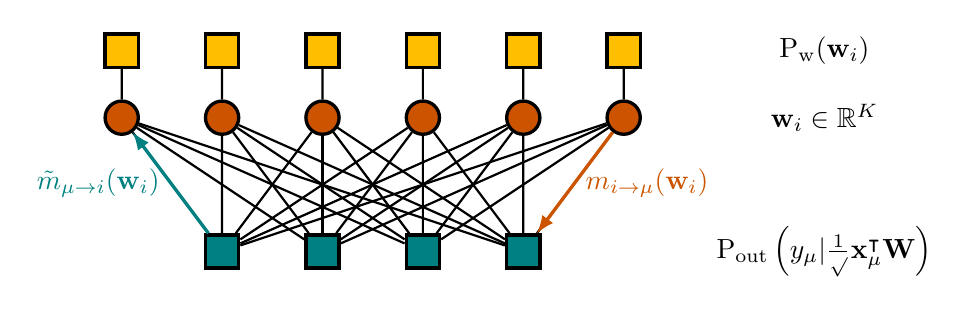
\begin{tikzpicture}[scale=0.85, auto, swap]
			    \foreach \i in {1,...,6}
			        \node[var] (X\i) at (1.5*\i,0) {};
			    \node at (12, 0) {$ \vec{w}_i \in \bbR^K $};
			
			    \foreach \mu in {1,...,4}
			        \node[inter] (Y\mu) at (1.5+1.5*\mu,-2) {};
			    \foreach \i in {1,...,6}
			        \foreach \mu in {1,...,4}
			            \path[edge] (X\i) -- (Y\mu);
			    \node at (10, -2) {};
			    \node (F) at (12, -2) {$ \rP_{\out}\(y_\mu | \frac{1}{\sqrt{\ndim}} \vec{x}_\mu^\intercal \mat{W} \) $};			
			    \foreach \i in {1,...,6} {
			        \node[field] (P\i) at (1.5*\i,1) {};
			        \path[edge] (X\i) -- (P\i);
			    }
			    \node at (12, 1) {$ \rP_\w(\vec{w}_i) $};
			    \path[-latex, teal, very thick] (Y1) edge node[left]{$\td{m}_{\mu \to i}(\vec{w}_i)$} (X1);
			    \path[-latex, burntorange, very thick] (X6) edge node[right]{$m_{i \to \mu}(\vec{w}_i)$} (Y4);
			\end{tikzpicture}
			\caption{Factor graph representation of the joint distribution for committee machines.}
			\label{fig:amp:factor_graph_committee}
			\end{figure}
		In the following, we attach a set of \emph{messages} $\{m_{i\to \mu},\tilde{m}_{\mu \to i}\}_{i=1..n}^{\mu=1..m}$ to the edges of this bipartite factor graph. These messages correspond to the marginal probabilities of $\vec{w}_i \in \bbR^K$ if we remove the edges $(i \to \mu)$ or $(\mu \to i)$. 
			We define the auxiliary variable $\vec{z}_\indsamples = \frac{1}{\sqrt{\ndim}}\vec{x}_\indsamples^\intercal \mat{W} \in \bbR^K $ which is $\Theta(1)$ thanks to the pre-factor rescaling $1/\sqrt{d}$. This scaling is crucial as it allows the BP equations to hold true even though the factor graph is not tree-like and is instead fully connected with short loops.
				
\subsection{Belief Propagation equations}		
		The BP equations (also called the sum-product equations) for $\vec{w}_i=(w_{ik})_{k=1..K} \in \bbR^K$ on the factor graph \Fig\ref{fig:amp:factor_graph_committee} can be formulated as:
			\begin{align}
					m_{i\to \mu}^{t+1} (\vec{w}_i) &= \displaystyle \frac{1}{\mZ_{i\to \mu}} \rP_\w (\vec{w}_i) \prod\limits_{\nu \neq \mu}^\nsamples \tilde{m}_{\nu \to i}^t (\vec{w}_i) \label{appendix:amp:bp_equations_committee} \\
					\tilde{m}_{\mu \to i}^t (\vec{w}_i) &=  \displaystyle \frac{1}{\mZ_{\mu \to i}} \int_{\bbR^K} \prod\limits_{j\neq i}^\ndim \d \vec{w}_j ~ \rP_\out \(y_{\mu} |  \frac{1}{\sqrt{\ndim}} \sum_{j=1}^\ndim  x_{\mu j}\vec{w}_{j} \)  m_{j \to \mu}^t (\vec{w}_j )\,, \nonumber
			\end{align}
		The BP equations assume that incoming messages are independent. Hence these equations are exact on a tree (no loop), but they remain exact if "correlations decrease fast enough / long loops". We assume in the following that the hypothesis is true in our model.\\
										
\subsection{Relaxed Belief Propagation equations}
		The idea of the relaxed BP equations is to simply expand in the limit $\ndim \to \infty$ the set of $\Theta(\ndim^2)$ messages $\td{m}$ of the BP equations in \eqref{appendix:amp:bp_equations_committee} before plugging them in $m$. Truncating the expansion and keeping only terms of order $\Theta\(1/\ndim\)$, messages become \emph{Gaussian}.
			Hence messages are therefore parametrized only by the mean $\hat{\vec{w}}_{i\to \mu}^t$ and the covariance matrix $\hat{\mat{C}}_{i\to \mu}^t$ of the marginal distribution at time $t$:
			\begin{align}
			\begin{aligned}
				\hat{\vec{w}}_{i\to \mu}^t &\equiv \displaystyle \int_{\bbR^K} \d \vec{w}_i ~
					 m_{i \to \mu}^t (\vec{w}_i) ~ \vec{w}_i \spacecase
					 \hat{\mat{C}}_{i \to \mu}^t &\equiv \displaystyle \int_{\bbR^K} \d \vec{w}_i ~
					 m_{i \to \mu}^t (\vec{w}_i) ~ \vec{w}_i \vec{w}_i^\intercal - \hat{\vec{w}}_{i \to \mu}^t(\hat{\vec{w}}_{i \to \mu}^t)^\intercal
			\end{aligned}
			\label{appendix:amp:committee:what_chat}
			\end{align}
		To decouple the argument of $\rP_{\out}$, we first by introducing its Fourier transform $\hat{\rP}_{\out}$ according to
			\begin{align*}
			&\rP_\out \(y_{\mu} |  \frac{1}{\sqrt{\ndim}} \sum_{j=1}^\ndim  x_{\mu j}\vec{w}_{j} \) = \frac{1}{(2\pi)^{K/2}}\\
			& \qquad \qquad  \times \int_{\bbR^K} \d \bxi \exp\( i \bxi^\intercal \( \displaystyle \frac{1}{\sqrt{\ndim}} \sum_{j=1}^\ndim  x_{\mu j}\vec{w}_{j}\) \hat{\rP}_{\out}(y_{\mu} , \bxi )    \).	
			\end{align*}
			Injecting this representation in the BP equations, \eqref{appendix:amp:bp_equations_committee} becomes:
			\begin{align}
			&\tilde{m}_{\mu \to i}^t (\vec{w}_i ) = 
			\frac{1}{(2\pi)^{K/2}\mZ_{\mu\to i} }
			\int_{\bbR^K} \d \bxi ~ \hat{\rP}_{\out}(y_{\mu} , \bxi) ~ 
			\exp\(i  \bxi^\intercal \frac{1}{\sqrt{\ndim}} x_{\mu i} \vec{w}_i \)\nonumber\\
			 &\qquad \times\prod\limits_{j\neq i}^\ndim \underbrace{\int_{\bbR^K} \d \vec{w}_j ~
					 m_{j \to \mu}^t (\vec{w}_j ) ~ \exp\( i  \bxi^\intercal \frac{1}{\sqrt{\ndim}} x_{\mu j} \vec{w}_j ) \)}_{\equiv I_j}\label{appendix:amp:bp_equations_committe:mtilde}
			\end{align}
			In the limit $\ndim \to \infty$ the term $I_j$ can be easily expanded and expressed using $\hat{\vec{w}}$ and $\hat{\mat{C}}$ in \eqref{appendix:amp:committee:what_chat}:
			\begin{align*}
			 I_j &= \int_{\bbR^K} \d \vec{w}_j ~
					 m_{j \to \mu}^t (\vec{w}_j ) ~ \exp\( i \frac{x_{\mu j}}{\sqrt{\ndim}} \bxi^\intercal \vec{w}_j ) \) \\
					 & \simeq  \exp\( i \frac{x_{\mu j}}{\sqrt{\ndim}} \bxi^\intercal  \hat{\vec{w}}_{j\to \mu}^t -  \frac{1}{2} \frac{x_{\mu j}^2}{\ndim}  \bxi^\intercal \hat{\mat{C}}_{j\to \mu}^t  \bxi \).
			\end{align*} 
			Finally using the inverse Fourier transform:
			\begin{align*}
			&\tilde{m}_{\mu \to i}^t (\vec{w}_i ) = 
			\frac{1}{(2\pi)^{K/2} \mZ_{\mu \to i}}
			\int_{\bbR^K} \d \vec{z} \rP_{\out}(y_\mu | \vec{z} ) 
			\int_{\bbR^K} \d \bxi  
			e^{-i \bxi^\intercal \vec{z}}
			e^{ i x_{\mu i} \bxi^\intercal \vec{w}_i} \\
			&\qquad\qquad\qquad\times\prod\limits_{j\neq i}^\ndim \exp\( i \frac{x_{\mu j}}{\sqrt{\ndim}} \bxi^\intercal \hat{\vec{w}}_{j\to \mu}^t -  \frac{1}{2}\frac{x_{\mu j}^2}{\ndim} \bxi^\intercal \hat{\mat{C}}_{j\to \mu}^t \bxi \) \\
			&= \frac{1}{(2\pi)^{K} \mZ_{\mu\to i}}
			\int_{\bbR} \d \vec{z} ~ \rP_{\out}(y_\mu | \vec{z} )\\
			& \qquad\qquad \int_{\bbR^K} \d \bxi ~ e^{-i \bxi^\intercal \vec{z}}
			e^{ i x_{\mu i} \bxi^\intercal \vec{w}_i} e^{i \sum\limits_{j\neq i}^\ndim\frac{x_{\mu j}}{\sqrt{\ndim}}  \bxi^\intercal \hat{\vec{w}}_{j\to \mu}^t } e^{-  \frac{1}{2} \sum\limits_{j\neq i}^\ndim\frac{x_{\mu j}^2}{\ndim}  \bxi^\intercal  \hat{\mat{C}}_{j \to \mu }^t \bxi} \\
			&= \frac{1}{(2\pi)^K \mZ_{\mu\to i}} \int_{\bbR^K} \d \vec{z} ~ \rP_{\out}(y_\mu | \vec{z}) \\ 
			& \qquad \quad \times \sqrt{\frac{(2\pi)^K}{\det{V_{\mu \to i}^t}}} \underbrace{e^{-\frac{1}{2} \( \vec{z} -\frac{x_{\mu i}}{\sqrt{\ndim}} \vec{w}_i -\bomega_{\mu \to i}^t \)^\intercal (\mat{V}_{\mu \to i}^t)^{-1} \( \vec{z} -\frac{x_{\mu i}}{\sqrt{\ndim}} \vec{w}_i -\bomega_{\mu \to i}^t \)}}_{\equiv H_{\mu \to i}}\,,
			\end{align*}
			where we defined the mean and variance, depending on the node $i$:
			\begin{align*}
				\bomega_{\mu \to i}^t &\equiv  \frac{1}{\sqrt{\ndim}} \sum\limits_{j\neq i}^\ndim x_{\mu j}  \hat{\vec{w}}_{j\to \mu}^t \,, &&
				\mat{V}_{\mu \to i}^t \equiv  \frac{1}{\ndim} \sum\limits_{j\neq i}^\ndim x_{\mu j}^2  \hat{\mat{C}}_{j \to \mu}^t\,.
			\end{align*}
			Again, in the limit $\ndim\to \infty$, the term $H_{\mu \to i}$ can be expanded as
			\begin{align*}
				H_{\mu \to i} &\simeq  e^{-\frac{1}{2} \( \vec{z} -\bomega_{\mu \to i}^t \)^\intercal (\mat{V}_{\mu \to i}^t)^{-1} \( \vec{z} -\bomega_{\mu \to i}^t \) } \\
				& \times 
				\( 1 + \frac{x_{\mu i}}{\sqrt{\ndim}} \vec{w}_i^\intercal (\mat{V}_{\mu \to i}^t)^{-1} (\vec{z} -\bomega_{\mu \to i}^t) -\frac{1}{2}\frac{x_{\mu i}^2}{\ndim} \vec{w}_i^\intercal (\mat{V}_{\mu \to i}^t)^{-1} \vec{w}_i \right.\\
			& \left. + \frac{1}{2} \frac{x_{\mu i}^2}{\ndim} \vec{w}_i^\intercal (\mat{V}_{\mu \to i}^t)^{-1} (\vec{z} -\bomega_{\mu \to i}^t) (\vec{z} - \bomega_{\mu \to i}^t)^\intercal  (\mat{V}_{\mu \to i}^t)^{-1} \vec{w}_i \).
			\end{align*}
			Putting all pieces together, the message $\tilde{m}_{\mu \to i}$ can be expressed using definitions of $\vec{f}_\out$ and $\partial_{\omega} \vec{f}_\out$ in \App\ref{appendix:definitions:updates:committee}. We finally obtain
			\begin{align*}
			&\tilde{m}_{\mu  \to i}^t (\vec{w}_i ) \sim \frac{1}{\mZ_{\mu \to i}} \left \{1 +  \frac{x_{\mu i}}{\sqrt{\ndim}} \vec{w}_{i}^\intercal  \vec{f}_\out (y_{\mu}, \bomega_{\mu \to i}^t, \mat{V}_{\mu \to i}^t) \right. \\
			&\left. \qquad\qquad \qquad\qquad + \frac{1}{2} \frac{x_{\mu i}^2}{\ndim} \vec{w}_{i}^\intercal \vec{f}_\out  \vec{f}_\out^\intercal (y_{\mu}, \bomega_{\mu \to i}^t, \mat{V}_{\mu \to i}^t) \vec{w}_{i} \right. \\
			& \left.\qquad\qquad \qquad\qquad  + \frac{1}{2} \frac{x_{\mu i}^2}{\ndim} \vec{w}_{i}^\intercal  \partial_\bomega \vec{f}_\out(y_{\mu}, \bomega_{\mu \to i}^t, \mat{V}_{\mu \to i}^t)  \vec{w}_{i}
			\right\}\\
			&= \frac{1}{\mZ_{\mu \to i}} \left\{ 1 + \vec{w}_{i}^\intercal  \vec{b}_{\mu \to i}^t +\frac{1}{2}  \vec{w}_{i}^\intercal  \vec{b}_{\mu \to i}^t (\vec{b}_{\mu \to i}^t)^\intercal  (\vec{w}_{i}) -\frac{1}{2} \vec{w}_{i}^\intercal  \mat{A}_{\mu \to i}^t w_{i} \right\} \\
			&=\sqrt{\frac{\det{\mat{A}_{\mu \to i}^t}}{(2\pi)^K}} e^{-\frac{1}{2}\(\vec{w}_{i}^\intercal  - (\mat{A}_{\mu \to i}^t)^{-1}\vec{b}_{\mu \to i}^t \)^\intercal  \mat{A}_{\mu \to i}^t\(\vec{w}_{i}^\intercal  - (\mat{A}_{\mu \to i}^t)^{-1}\vec{b}_{\mu \to i}^t \) }
			\end{align*}
			with the following definitions of $\mat{A}_{\mu \to i}$ and $\vec{b}_{\mu \to i}$
			\begin{align*}
					\vec{b}_{\mu \to i}^t &\equiv  \frac{x_{\mu i}}{\sqrt{\ndim}} \vec{f}_\out (y_{\mu}, \bomega_{\mu \to i}^t, \mat{V}_{\mu \to i}^t) \,,\\
					\mat{A}_{\mu \to i}^t &\equiv - \frac{x_{\mu i}^2}{\ndim}  \partial_\bomega \vec{f}_\out(y_{\mu}, \bomega_{\mu \to i}^t, \mat{V}_{\mu \to i}^t)\,.
			\end{align*}
			The set of BP equations can finally be closed over the Gaussian messages $\{m_{i\to \mu}\}_{i=1..\ndim}^{\mu=1..\nsamples}$ according to
			\begin{align*}
				 m_{i\to \mu}^{t+1} (\vec{w}_i) &= \frac{1}{\mZ_{i\to \mu}} \rP_\w (\vec{w}_i) \prod\limits_{\nu \neq \mu}^\nsamples \sqrt{\frac{\det{\mat{A}_{\nu \to i}^t}}{(2\pi)^K}} \\
				 & \qquad \qquad \qquad \times e^{-\frac{1}{2}\(\vec{w}_{i} - (\mat{A}_{\nu \to i}^t)^{-1}\vec{b}_{\nu \to i}^t \)^\intercal  \mat{A}_{\nu \to i}^t\(w_{i} - (\mat{A}_{\nu \to i}^t)^{-1}\vec{b}_{\nu \to i}^t \) }.
			\end{align*}
			In the end, computing the mean and variance of the product of Gaussians, the messages are updated using $\vec{f}_\w$ and $\partial_\bgamma \vec{f}_\w$, defined in \App\ref{appendix:definitions:updates:committee}, according to
			\begin{align*}
				\hat{\vec{w}}_{i\to \mu}^{t+1} &= \vec{f}_\w( \bgamma_{\mu \to i}^t, \bLambda_{\mu \to i}^t  )\,,
				&& \hat{\mat{C}}_{i \to \mu}^{t+1}=\partial_\bgamma \vec{f}_\w( \bgamma_{\mu \to i}^t, \bLambda_{\mu \to i}^t )\,,
			\end{align*}
			with
			\begin{align*}
				\bgamma_{\mu \to i}^t &= \sum\limits_{\nu \ne \mu}^\nsamples  \vec{b}_{\nu \to i}^t \,, 
				&& \bLambda_{\mu \to i}^t = \sum\limits_{\nu \ne \mu}^\nsamples  \mat{A}_{\nu \to i}^t \,.
			\end{align*}
			
		\paragraph{Summary of the rBP equations}
			In the end, the \aclink{rBP} equations are simply the following set of equations:
			\begin{align}
			\label{appendix:amp:committee:relaxed_bp_summary}
			\begin{aligned}
				\hat{\vec{w}}_{i\to \mu}^{t+1} &= \vec{f}_\w(\bgamma_{\mu \to i}^t,\bLambda_{\mu \to i}^t )\,, 
				&&\hat{\mat{C}}_{i \to \mu}^{t+1} = \partial_\bgamma \vec{f}_\w(\bgamma_{\mu \to i}^t, \bLambda_{\mu \to i}^t)  \\
				\bgamma_{\mu \to i}^t &=  \sum\limits_{\nu \ne \mu}^\nsamples  \vec{b}_{\nu \to i}^t \,, 
				&& \bLambda_{\mu \to i}^t =  \sum\limits_{\nu \ne \mu}^\nsamples  \mat{A}_{\nu \to i}^t   \\
			\vec{b}_{\mu \to i}^t &=  \frac{x_{\mu i}}{\sqrt{\ndim}} \vec{f}_\out (y_{\mu}, \bomega_{\mu \to i}^t, \mat{V}_{\mu \to i}^t) \,, \\ 
			\mat{A}_{\mu \to i}^t &= - \frac{x_{\mu i}^2}{\ndim}  \partial_\bomega \vec{f}_\out(y_{\mu}, \bomega_{\mu \to i}^t, \mat{V}_{\mu \to i}^t) \\
				\bomega_{\mu \to i}^t &= \sum\limits_{j\neq i}^\ndim\frac{x_{\mu j}}{\sqrt{\ndim}}   \hat{\vec{w}}_{j\to \mu}^t\,,
				&& \mat{V}_{\mu \to i}^t = \sum\limits_{j\neq i}^\ndim\frac{x_{\mu j}^2}{\ndim} \hat{\mat{C}}_{j\to \mu}^t\,.
			\end{aligned}
			\end{align}
			
\subsection{AMP algorithm}
\label{appendix:amp:derivation:amp_eqs}
	The \aclink{rBP} equations \eq\eqref{appendix:amp:committee:relaxed_bp_summary} contains $\Theta(\ndim^2)$ messages. However all the messages depend weakly on the target node. The missing message is negligible in the limit $\ndim \to \infty$, that allows us to expand the \aclink{rBP} around the \emph{full} messages:
			\begin{align}
			\begin{aligned}
				\bomega_{\mu}^t &\equiv \sum\limits_{j = 1}^\ndim\frac{x_{\mu j}}{\sqrt{\ndim}}   \hat{\vec{w}}_{j\to \mu}^t\,, 
				&& \mat{V}_{\mu}^t \equiv \sum\limits_{j=1}^\ndim  \frac{x_{\mu j}^2}{\ndim}  \hat{\mat{C}}_{j\to \mu}^t \\
				\bgamma_{i}^t & \equiv  \sum\limits_{\mu =1}^\nsamples  \vec{b}_{\mu \to i}^t \,,
				&& \bLambda_{i}^t \equiv  \sum\limits_{\mu =1}^\nsamples  \mat{A}_{\mu \to i}^t \,.
			\end{aligned}		
			\end{align}
			By completing the sum, we naturally remove the target node dependence and reduce the set of messages to $\Theta(\ndim)$. Let us now perform the expansion of the \aclink{rBP} messages.
	
	\paragraph{Partial covariance $\vec{f}_\w$: $\bLambda_{\mu \to i}^t$}
			\begin{align*}
				&\bLambda_{\mu \to i}^t =  \sum\limits_{\nu \ne \mu}^\nsamples  \mat{A}_{\nu \to i}^t 
				=  \sum\limits_{\nu =1 }^\nsamples  \mat{A}_{\nu \to i}^t - \mat{A}_{\mu \to i}^t  \\
				&= \bLambda_{i}^t - \mat{A}_{\mu \to i}^t = \bLambda_{i  }^t + \Theta\(\frac{1}{\ndim} \) \,.
			\end{align*}
			
	\paragraph{Partial mean $\vec{f}_\w$: $\bgamma_{\mu \to i}^t$}
			\begin{align*}
				\bgamma_{\mu \to i}^t &= \sum\limits_{\nu \ne \mu}^\nsamples  \vec{b}_{\nu \to i}^t  = \sum\limits_{\nu =1}^\nsamples  \vec{b}_{\nu \to i}^t -  \vec{b}_{\mu \to i}^t = \bgamma_{i}^t - \vec{b}_{\mu \to i}^t + \Theta\(\frac{1}{\ndim}\)\,.
			\end{align*}
			
	\paragraph{Mean $\hat{\vec{w}}_{i\to \mu}^{t+1}$ update}
			\begin{align*}
				\hat{\vec{w}}_{i\to \mu}^{t+1} &= \vec{f}_\w(\bgamma_{\mu \to i}^t , \bLambda_{\mu \to i}^t ) = \vec{f}_\w\(\bgamma_{i}^t - \vec{b}_{\mu \to i}^t,  \bLambda_{i}^t \) + \Theta\(\frac{1}{\ndim}\)\\
				&= \vec{f}_\w\(\bgamma_{i}^t, \bLambda_{i}^t \) -  \partial_\bgamma \vec{f}_\w \(\bgamma_{i}^t, \bLambda_{i}^t\) \vec{b}_{\mu \to i}^t  + \Theta\( \frac{1}{\ndim} \) \\
				&= \hat{\vec{w}}_{i}^{t+1} - \hat{\mat{C}}_{i}^{t+1} \vec{b}_{\mu \to i}^t  + \Theta\( \frac{1}{\ndim} \)\\
				&= \hat{\vec{w}}_{i}^{t+1} - \frac{x_{\mu i}}{\sqrt{\ndim}} \hat{\mat{C}}_{i}^{t+1} \vec{f}_\out (y_{\mu}, \bomega_{\mu}^t, \mat{V}_{\mu}^t) + \Theta\( \frac{1}{\ndim} \)\,.
			\end{align*}
			where we defined the prior updates
			\begin{align*}
				\hat{\vec{w}}_{i}^{t+1} &\equiv \vec{f}_\w\( \bgamma_{i}^t, \bLambda_{i}^t \)\,, && \hat{\mat{C}}_{i}^{t+1}\equiv \partial_\bgamma  \vec{f}_\w\(\bgamma_{i}^t, \bLambda_{i}^t \)\,,
			\end{align*}
			and used the fact that $\vec{b}_{\mu \to i}^t \simeq \frac{x_{\mu i}}{\sqrt{\ndim}} \hat{\mat{C}}_{i}^{t+1} \vec{f}_\out (y_{\mu}, \bomega_{\mu}^t, \mat{V}_{\mu}^t) $ by expanding the equation over $\vec{b}_{\mu \to i}^t$ in \eqref{appendix:amp:committee:relaxed_bp_summary}.
			
		\paragraph{Covariance $\hat{\mat{C}}_{i\to \mu}^{t+1}$ update}
			\begin{align*}
				\hat{\mat{C}}_{i\to \mu}^{t+1} &= \partial_\bgamma \vec{f}_\w(\bgamma_{\mu \to i}^t, \bLambda_{\mu \to i}^t) \\
				&\simeq \partial_\bgamma \vec{f}_\w(\bgamma_{i}^t, \bLambda_{i}^t)  + \Theta\( \frac{1}{\sqrt{\ndim}} \) = \hat{\mat{C}}_{i}^{t+1} + \Theta\( \frac{1}{\sqrt{\ndim}} \) \,.
			\end{align*}
		
		\paragraph{Channel update function $\vec{f}_\out(y_{\mu}, \bomega_{\mu \to i}^t, \mat{V}_{\mu \to i}^t)$}
	
			\begin{align*}
				&\vec{f}_\out(y_{\mu}, \bomega_{\mu \to i}^t, \mat{V}_{\mu \to i}^t) = \vec{f}_\out \(y_{\mu}, \bomega_{\mu}^t - \frac{x_{\mu i}}{\sqrt{\ndim}}   \hat{\vec{w}}_{i\to \mu}^t, \mat{V}_{\mu}^t - \frac{x_{\mu i}^2}{\ndim}   \hat{\mat{C}}_{i \to l}^t \)\\
				&= \vec{f}_\out \( y_{\mu}, \bomega_{\mu}^t, \mat{V}_{\mu}^t \) - \frac{x_{\mu i}}{\sqrt{\ndim}} \partial_\bomega \vec{f}_\out\( y_{\mu}, \bomega_{\mu}^t, \mat{V}_{\mu}^t \)   \underbrace{\hat{\vec{w}}_{i\to \mu}^t}_{=\hat{\vec{w}}_{i}^t + \Theta\( \frac{1}{\sqrt{\ndim}}\)} + \Theta\( \frac{1}{\ndim}\)\\
				&= \vec{f}_\out \( y_{\mu}, \bomega_{\mu}^t, \mat{V}_{\mu}^t \)-\frac{x_{\mu i}}{\sqrt{\ndim}} \partial_\bomega \vec{f}_\out\( y_{\mu}, \bomega_{\mu}^t, \mat{V}_{\mu}^t \)   \hat{\vec{w}}_{i}^t + \Theta\( \frac{1}{\ndim}\)\,.
			\end{align*}
			
		\paragraph{Covariance $\vec{f}_\out$: $\mat{V}_{\mu}^t$}
			\begin{align*}
			 \mat{V}_{\mu}^t &\equiv \sum\limits_{j=1}^\ndim  \frac{x_{\mu j}^2}{\ndim}  \hat{\mat{C}}_{j\to \mu}^t = \sum\limits_{j=1}^\ndim  \frac{x_{\mu j}^2}{\ndim}  \hat{\mat{C}}_{j\to \mu}^t + \Theta \( \frac{1}{\ndim^{3/2}}\) \,.
			\end{align*}
			
		\paragraph{Mean $\vec{f}_\out$: $\bomega_{\mu}^t$}
			\begin{align*}
				\bomega_{\mu}^t &= \sum\limits_{i = 1}^{\ndim} \frac{x_{\mu i}}{\sqrt{\ndim}}   \hat{\vec{w}}_{i\to \mu}^t \\
				&= \sum\limits_{i = 1}^{\ndim} \frac{x_{\mu i}}{\sqrt{\ndim}} \(\hat{\vec{w}}_{i}^t - x_{\mu i} \hat{\mat{C}}_{i}^t \vec{f}_\out (y_{\mu}, \bomega_{\mu}^{t-1}, \mat{V}_{\mu}^{t-1}) + \Theta\( \frac{1}{\ndim} \)  \) \\
				&= \sum\limits_{i = 1}^{\ndim} \frac{x_{\mu i}}{\sqrt{\ndim}} \hat{\vec{w}}_{i}^t -   \sum\limits_{i = 1}^{\ndim} \frac{x_{\mu i}^2}{\ndim}\hat{\mat{C}}_{i}^t \vec{f}_\out ( y_{\mu}, \bomega_{\mu}^{t-1}, \mat{V}_{\mu}^{t-1}) + \Theta \( \frac{1}{\ndim^{3/2}}\)\,.
			\end{align*}
			
		\paragraph{Covariance $\vec{f}_\w$: $\bLambda_{i}^t$}
			\begin{align*}
			\bLambda_{i}^t &\equiv  \sum\limits_{\mu =1}^\nsamples  \mat{A}_{\mu \to i}^t  =   \sum\limits_{\nu =1}^\nsamples - \frac{x_{\mu i}^2}{\ndim}  \partial_\bomega \vec{f}_\out(y_{\mu}, \bomega_{\mu \to i}^t, \mat{V}_{\mu \to i}^t)   \\
			&=   \sum\limits_{\mu =1}^\nsamples - \frac{x_{\mu i}^2}{\ndim}  \partial_\bomega \vec{f}_\out(y_{\mu}, \bomega_{\mu}^t, \mat{V}_{\mu}^t)  + \Theta\( \frac{1}{\ndim^{3/2}}\) \,.
			\end{align*}
			
		\paragraph{Mean $\vec{f}_\w$: $\bgamma_{i}^t$}
			\begin{align*}
			\bgamma_{i}^t &=  \sum\limits_{\mu =1}^\nsamples  \vec{b}_{\mu \to i}^t =  \sum\limits_{\mu =1}^\nsamples   \frac{x_{\mu i}}{\sqrt{\ndim}} \vec{f}_\out (y_{\mu}, \bomega_{\mu \to i}^t, \mat{V}_{\mu \to i}^t) \\
			&= \sum\limits_{\mu =1}^\nsamples    \frac{x_{\mu i}}{\sqrt{\ndim}} \vec{f}_\out (y_{\mu}, \bomega_{\mu}^t, \mat{V}_{\mu}^t) \\
			& \qquad -\frac{x_{\mu i}^2}{\ndim} \partial_\bomega \vec{f}_\out (y_{\mu}, \bomega_{\mu}^t, \mat{V}_{\mu}^t) \hat{\vec{w}}_{i}^t  + \Theta\(\frac{1}{\ndim^{3/2}} \)\,.
			\end{align*}
			
		\subsubsection*{Summary - AMP algorithm}
		We finally obtain the AMP algorithm as a reduced set of $\Theta(\ndim)$ messages in \Alg\ref{alg:appendix:amp:committee_machine}.
			\begin{algorithm} 
			\begin{algorithmic}
			    \STATE {\bfseries Input:} vector $\vec{y} \in \bbR^\nsamples$ and matrix $\mat{X}\in \bbR^{\nsamples \times \ndim}$:
			    \STATE \emph{Initialize}: $\hat{\vec{w}}_i$, $\vec{f}_{\out,\mu} \in \bbR^K$ and $\hat{\mat{V}}_i$, $\partial_{\bomega} \vec{f}_{\out, \mu} \in \bbR^{K\times K}$ for $ 1 \leq i \leq \ndim $ and $ 1 \leq \mu \leq \nsamples $ at $t=0$.
			    \REPEAT   
			    \STATE \noindent Channel: Update the mean $\omega_{\mu} \in \bbR^K$ and variance $V_{\mu}\in \bbR^{K\times K}$: \spacecase
			    \indent $\mat{V}_{\mu}^t = \sum\limits_{i=1}^\ndim  \frac{x_{\mu j}^2}{\ndim}  \hat{\mat{C}}_{i}^t $\\ 
			    \indent $\bomega_{\mu}^t = \sum\limits_{i = 1}^{\ndim} \frac{x_{\mu i}}{\sqrt{\ndim}} \hat{\vec{w}}_{i}^t -   \mat{V}_{\mu}^t \vec{f}_{\out,\mu}^{t-1}$\,, \\
			    \STATE \noindent Update $\vec{f}_{\out, \mu}$ and $\partial_\bomega \vec{f}_{\out,\mu}$: \spacecase
			    $\vec{f}_{\out,\mu}^t = \vec{f}_\out \( y_{\mu}, \bomega_{\mu}^t, \mat{V}_{\mu}^t \)$\,, $ \partial_\bomega \vec{f}_{\out^,\mu}^t = \partial_\bomega\vec{f}_\out \( y_{\mu}, \bomega_{\mu}^t, \mat{V}_{\mu}^t \)$ \spacecase
			    \STATE \noindent Prior: Update the mean $\bgamma_i \in \bbR^K$ and variance $\bLambda_i \in \bbR^{K\times K}$:\spacecase
			    $ \bLambda_{i}^t =  \sum\limits_{\mu =1}^\nsamples - \frac{x_{\mu i}^2}{\ndim}  \partial_\bomega \vec{f}_{\out, \mu} $\spacecase
			    $\bgamma_i^t = \sum\limits_{\mu =1}^\nsamples    \frac{x_{\mu i}}{\sqrt{\ndim}} \vec{f}_{\out,\mu} + \bLambda_{i}^t \hat{\vec{w}}_{i}^t $\,,
			    \STATE Update the estimated marginals $\hat{\vec{w}}_i \in \bbR$ and $\hat{\mat{C}}_i \in \bbR^+$: \spacecase
			   $\hat{\vec{w}}_{i}^{t+1}= \vec{f}_\w\( \bgamma_{i}^t, \bLambda_{i}^t \)$\,, $\hat{\mat{C}}_{i}^{t+1}= \partial_\bgamma  \vec{f}_\w\(\bgamma_{i}^t, \bLambda_{i}^t \)$\spacecase
			    \STATE ${t} \leftarrow {t} + 1$ 
			    \UNTIL{Convergence on
			    $\hat{\vec{w}}_i$, $\hat{\mat{C}}_i$.} 
			    \STATE {\bfseries Output:}
			    $\{\hat{\vec{w}_i}\}_{i=1}^\ndim$ and $\{\hat{\mat{C}}_i\}_{i=1}^\ndim$.
			\end{algorithmic}
			\caption{Approximate Message Passing algorithm for committee machines.}
  			\label{alg:appendix:amp:committee_machine}
			\end{algorithm}
			
\subsection{State evolution equations of AMP}
\label{appendix:amp:derivation:se_eqs}
In this section we derive the behavior of the AMP algorithm in  \Alg\ref{alg:appendix:amp:committee_machine} in the thermodynamic limit $\ndim \to \infty$. This average asymptotic behavior can be tracked with some overlap parameters at time $t$, $\mat{m}^t$, $\mat{q}^t$, $\bSigma^t$, that respectively measure the correlation of the AMP estimator with the ground truth, the norms of student and teacher weights, the estimator variance and the second moment of the teacher network $ \brho_{\w^\star}$, defined by
\begin{align}
\begin{aligned}
	\mat{m}^t &\equiv \displaystyle \EE \lim_{\ndim \to \infty} \frac{1}{\ndim}\hat{\mat{W}}^{t \intercal} \hat{\mat{W}}^{\star} \,, 
	&& \mat{q}^t  \equiv \displaystyle \EE \lim_{\ndim \to \infty} \frac{1}{\ndim} \hat{\mat{W}}^{t \intercal} \hat{\mat{W}}^{t}  \,, \\ 
	\bSigma^t & \equiv \displaystyle \EE \lim_{\ndim \to \infty} \frac{1}{\ndim} \sum_{i=1}^\ndim \hat{\mat{C}}_{i}^{t} \,, &&
	\brho_{\w^\star} \equiv \displaystyle \EE \lim_{\ndim \to \infty} \frac{1}{\ndim} \mat{W}^{\star \intercal} \mat{W}^{\star} \,,
\end{aligned}
\label{appendix:amp:derivation:se_eqs:overlaps}
\end{align}
where the expectation is over ground truth signals $\mat{W}^\star$ and input data $\mat{X}$. The aim is to derive the asymptotic behavior of these overlap parameters, called \aclink{SE}. The idea is simply to compute the overlap distributions starting with the set of \aclink{rBP} equations in \eqref{appendix:amp:committee:relaxed_bp_summary}.

\subsubsection{Messages distribution}
In order to get the asymptotic behavior of the overlap parameters, we first need to compute the distribution of $\mat{W}^{t+1}$ and, as a result, of the mean $\bgamma_{\mu \to i}^t$ and covariance $\bLambda_{\mu \to i}^t$. 
Recalling that under the BP assumption incoming messages are independent, the messages $\bomega_{\mu \to i}^t$ and $\vec{z}_{\mu}$ are the sum of independent variables and follow Gaussian distributions. 
However, these two variables are correlated and we need to compute correctly the covariance matrix.

To compute it, we will make use of different ingredients. 
First, we recall that in the \aclink{T-S} scenario, the output has been generated by a teacher such that $\forall \mu \in \lb \nsamples \rb,~ y_\mu = \varphi_{\out^\star} \(\frac{1}{\sqrt{\ndim}} \vec{x}_\mu^\intercal \mat{W}^\star \)$. By convenience, we define $\vec{z}_\mu \equiv \frac{1}{\sqrt{\ndim}} \vec{x}_\mu^\intercal \mat{W}^\star = \frac{1}{\sqrt{\ndim}} \sum_{i=1}^\ndim x_{\mu i} \vec{w}_i^\star $ and $z_{\mu \to i} \equiv  \frac{1}{\sqrt{\ndim}} \sum_{j \ne i}^\ndim x_{\mu j} \vec{w}_j^\star$. 
Second, in the case the input data are \aclink{i.i.d} Gaussian, we have $\EE_{\mat{X}}[x_{\mu i}] = 0 $ and $\EE_{\mat{X}} [x_{\mu i}^2] = 1$.

\paragraph{Partial mean $\vec{f}_\out$: $\bomega_{\mu \to i}^t$}
Let's compute the first two moments, using expansions of the \aclink{rBP} equations \eqref{appendix:amp:committee:relaxed_bp_summary}:
\begin{align*}
	&\EE\[ \bomega_{\mu \to i}^t\]  = \frac{1}{\sqrt{\ndim}} \sum\limits_{j \neq i}^\ndim  \EE_{\mat{X}} \[ x_{\mu j}\]   \EE \[ \hat{\vec{w}}_{j\to \mu}^t \] = \vec{0}\,, \\
	&\EE \[ \bomega_{\mu \to i}^t \( \bomega_{\mu \to i}^t\)^\intercal \]  = \frac{1}{\ndim} \sum\limits_{j \neq i}^\ndim \EE_{\mat{X}} \[ x_{\mu j}^2\]  \EE\[ \hat{\vec{w}}_{j\to \mu}^t \(\hat{\vec{w}}_{j\to \mu}^t\)^\intercal\]\\
	&= \frac{1}{\ndim} \sum\limits_{i=1}^\ndim \EE_{\mat{X}} \[ x_{\mu j}^2\]  \EE\[ \hat{\vec{w}}_{i}^t \(\hat{\vec{w}}_{i}\)^\intercal\] + \Theta\(\ndim^{-3/2}\)  \underlim{\ndim}{\infty} \mat{q}^t\,.
\end{align*}	

\paragraph{Hidden variable $\vec{z}_{\mu}$}
Let us compute the first moments of the hidden variable $\vec{z}_{\mu}$:
\begin{align*}
	\EE \[ \vec{z}_\mu \]  &= \frac{1}{\sqrt{\ndim}} \sum\limits_{i=1}^\ndim \EE_{\mat{X}}\[x_{\mu i}\] \EE_{\mat{W}^\star}\[\vec{w}_i^\star\]  = \vec{0} \,, \\
	\EE \[  \vec{z}_\mu  \vec{z}_\mu^\intercal \]  &= \frac{1}{\ndim} \sum\limits_{i=1}^\ndim \EE_{\mat{X}}\[x_{\mu i}^2\] \EE_{\mat{W}^\star}\[ \vec{w}_i^\star (\vec{w}_i^\star)^\intercal\] \underlim{\ndim}{\infty}\brho_{\w^\star} \,.
\end{align*}

\paragraph{Correlation between $\vec{z}_{\mu}$ and $\bomega_{\mu \to i}^t$}
The cross correlation is given by
\begin{align*}
	&\EE \[ \bomega_{\mu \to i}^t  \vec{z}_\mu^\intercal \] =  \frac{1}{\ndim} \sum\limits_{j\neq i, k=1 }^\ndim \EE_{\mat{X}} \[x_{\mu j} x_{\mu k} \]  \EE_{\mat{W}^\star} \[ \hat{\vec{w}}_{j\to \mu}^t (\vec{w}_{k}^\star)^\intercal \]  \\
	&=  \frac{1}{\ndim} \sum\limits_{j\neq i}^\ndim  \EE_{\mat{W}^\star} \[ \hat{\vec{w}}_{j\to \mu}^t (\vec{w}_{j}^\star)^\intercal \] = \frac{1}{\ndim} \sum\limits_{i}^\ndim  \EE_{\mat{W}^\star} \[ \hat{\vec{w}}_{i}^t (\vec{w}_{i}^\star)^\intercal \] + \Theta\(\ndim^{-3/2}\)\\
	& \qquad \underlim{\ndim}{\infty} \mat{m}^t \,.
\end{align*}
Hence asymptotically the random vector ($\vec{z}_\mu$, $\bomega_{\mu \to i}^t$) follow a multivariate Gaussian distribution with covariance matrix 
$ \mat{Q}^t = 
\begin{bmatrix}
    \brho_{\w^\star} & \mat{m}^t \\
    \mat{m}^t & \mat{q}^t  \\
\end{bmatrix} \in \bbR^{(2K) \times (2K)}$.
 
\paragraph{Partial variance $\vec{f}_\out$: $\mat{V}_{\mu \to i}$} 
$\mat{V}_{\mu \to i}$ concentrates around its mean:
\begin{align*}
	\EE \[ \mat{V}_{\mu \to i}^t \] &= \frac{1}{\ndim} \sum\limits_{j\neq i}^\ndim \EE_{\mat{X}} \[ x_{\mu j}^2 \] \hat{\mat{C}}_{j\to \mu}^t = \frac{1}{\ndim} \sum\limits_{i}^\ndim \hat{\mat{C}}_{i}^t + \Theta(\ndim^{-3/2}) \underlim{\ndim}{\infty} \bSigma^t \,.
\end{align*}

\paragraph{Ad-hoc overlaps}
Let us define some other ad-hoc order parameters, that will appear in the following:
\begin{align}
\begin{aligned}
		\hat{\mat{q}}^t & \equiv \alpha \EE_{\bomega,\vec{z}} \[ \vec{f}_{\out} (\varphi_{\out^\star}(\vec{z}), \bomega, \bSigma^t )^{\otimes 2}  \]  \,, \\
		 \hat{\mat{m}}^t &\equiv \alpha \EE_{\bomega, \vec{z}} \[ \partial_\vec{z} \vec{f}_{\out}(\varphi_{\out^\star}(\vec{z}), \bomega, \bSigma^t ) \]  \,, \\
		  \hat{\bchi}^t &\equiv \alpha \EE_{\bomega, \vec{z}} \[ - \partial_\bomega \vec{f}_{\out}(\varphi_{\out^\star}(\vec{z}), \bomega, \bSigma^t ) \] \,. \\
\end{aligned}
\end{align}

\paragraph{Partial mean $\vec{f}_\w$: $\bgamma_{\mu \to i}^t$} 
Using the expression $y_\nu = \varphi_{\out^\star}\( \vec{z}_{\nu \to i} + \frac{1}{\sqrt{\ndim}} x_{\nu i} \vec{w}_i^\star \)$ and expanding $\bgamma_{\mu \to i}^t$, we obtain
\begin{align*}
	&\bgamma_{\mu \to i}^t =  \sum\limits_{\nu \ne \mu}^\nsamples  \vec{b}_{\nu \to i}^t  =  \sum\limits_{\nu \ne \mu}^\nsamples  \frac{x_{\nu i}}{\sqrt{\ndim}} \vec{f}_\out \( y_\nu , \bomega_{\nu \to i}^t, \mat{V}_{\nu \to i}^t\) \\
	&=   \frac{1}{\sqrt{\ndim}} \sum\limits_{\nu \ne \mu}^\nsamples  x_{\nu i} \vec{f}_\out \( \varphi_{\out^\star}\( \vec{z}_{\nu \to i} \), \bomega_{\nu \to i}^t, \mat{V}_{\nu \to i}^t\) \\
	& + \frac{1}{\ndim} \sum\limits_{\nu \ne \mu}^\nsamples x_{\nu i}^2 \partial_\vec{z}\vec{f}_\out \( \varphi_{\out^\star}\( \vec{z}_{\nu \to i}\), \bomega_{\nu \to i}^t, \mat{V}_{\nu \to i}^t\) \vec{w}_i^\star \,.
\end{align*}
Thus, taking the average
\begin{align*}
	\EE\[ \bgamma_{\mu \to i}^t \] &= \vec{0} + \frac{1}{\ndim} \sum\limits_{\nu \ne \mu}^\nsamples \EE_{\vec{z}, \bomega} \[ \partial_\vec{z}\vec{f}_\out \( \varphi_{\out^\star}\( \vec{z}_{\nu \to i}\), \bomega_{\nu \to i}^t, \mat{V}_{\nu \to i}^t\) \] \vec{w}_i^\star \\
	& \underlim{\ndim}{\infty} \hat{\mat{m}}^t  \vec{w}_i^\star \,, \\
	\EE\[ (\bgamma_{\mu \to i}^t)^{\otimes 2} \] &= \frac{1}{\ndim} \sum\limits_{\nu \ne \mu}^\nsamples  \EE_{\vec{z}, \bomega}\[ \vec{f}_\out \( \varphi_{\out^\star}\( \vec{z}_{\nu \to i} \), \bomega_{\nu \to i}^t, \mat{V}_{\nu \to i}^t\)^{\otimes 2} \] \\
	& \underlim{\ndim}{\infty} \hat{\mat{q}}^t\,.
\end{align*}
Hence $ \bgamma_{\mu \to i}^t \sim  \hat{\mat{m}}^t \vec{w}_i^\star  + ( \hat{\mat{q}}^t)^{1/2}\bxi $ with $\bxi \sim \mN(\vec{0},\rI_K)$. 

\paragraph{Partial covariance $\vec{f}_\w$: $\bLambda_{\mu \to i}^t$}
\begin{align*}
	\bLambda_{\mu \to i}^t &= \sum\limits_{\nu \ne \mu}^\nsamples  \mat{A}_{\nu \to i}^t =  - \frac{1}{\ndim}  \sum\limits_{\nu \ne \mu}^\nsamples x_{\mu i}^2 \partial_\bomega \vec{f}_\out(y_{\nu}, \bomega_{\nu \to i}^t, \mat{V}_{\nu \to i}^t) \\
	& = - \frac{1}{\ndim}  \sum\limits_{\nu \ne \mu}^\nsamples x_{\mu i}^2 \partial_\bomega \vec{f}_\out( \varphi_{\out^\star}(\vec{z}_{\nu \to i}) , \bomega_{\nu \to i}^t, \mat{V}_{\nu \to i}^t)  + \Theta\(\ndim^{-3/2} \)
\end{align*}
and taking the average 
\begin{align*}
	\EE \[ \bLambda_{\mu \to i}^t\] &= - \frac{1}{\ndim}  \sum\limits_{\nu \ne \mu}^\nsamples \EE_{\vec{z}, \bomega}\[ \partial_\bomega \vec{f}_\out( \varphi_{\out^\star}(\vec{z}_{\nu \to i}) , \bomega_{\nu \to i}^t, \mat{V}_{\nu \to i}^t)\]\\
	& \qquad \underlim{\ndim}{\infty}  \hat{\bchi}^t\,,
\end{align*} 
so that in the thermodynamic limit $\bLambda_{\mu \to i}^t \sim \hat{\bchi}^t$.

\subsubsection{Summary of the SE - mismatched setting}
Using the definition of the overlaps in \eqref{appendix:amp:derivation:se_eqs:overlaps} at time $t+1$ and the message distributions, we finally obtain the set of \aclink{SE} equations of the AMP algorithm in \Alg\ref{alg:appendix:amp:committee_machine} in the mismatched setting:
\begin{align}
\begin{aligned}
	\mat{m}^{t+1} & \equiv \displaystyle \EE \lim_{\ndim \to \infty} \frac{1}{\ndim}\hat{\mat{W}}^{t+1 \intercal} \hat{\mat{W}}^{\star} = \EE_{\vec{w}^\star, \bxi} \[  \vec{f}_\w\( \hat{\mat{m}}^t \vec{w}^\star  + ( \hat{\mat{q}}^t)^{1/2}\bxi, \hat{\bchi}^t \) \vec{w}^{\star \intercal} \]  \,, \\
	\mat{q}^{t+1} &\equiv \displaystyle \EE \lim_{\ndim \to \infty} \frac{1}{\ndim} \hat{\mat{W}}^{t+1 \intercal} \hat{\mat{W}}^{t+1}= \EE_{\vec{w}^\star, \bxi} \[  \vec{f}_\w\( \hat{\mat{m}}^t \vec{w}^\star  + ( \hat{\mat{q}}^t)^{1/2}\bxi, \hat{\bchi}^t \)^{\otimes 2} \] \,, \\ 
	\bSigma^{t+1} & \equiv \displaystyle \EE \lim_{\ndim \to \infty} \frac{1}{\ndim} \sum_{i=1}^\ndim \hat{\mat{C}}_{i}^{t+1} = \EE_{\vec{w}^\star, \bxi} \[  \partial_\bgamma \vec{f}_\w\( \hat{\mat{m}}^t \vec{w}^\star  + ( \hat{\mat{q}}^t)^{1/2}\bxi, \hat{\bchi}^t \) \] \,,
\end{aligned}
\end{align}
and
\begin{align}
\begin{aligned}
	\hat{\mat{q}}^t &= \alpha\int_{\bbR^K} \int_{\bbR^K} \d \bomega ~ \d \vec{z} ~ \mN_{(\vec{z}, \bomega)}\(\vec{0}_{2K}, \mat{Q}^t \) \vec{f}_{\out} (\varphi_{\out^\star}(\vec{z}), \bomega, \bSigma^t )^{\otimes 2} \\
	\hat{\mat{m}}^t &= \alpha\int_{\bbR^K} \int_{\bbR^K} \d \bomega ~ \d \vec{z} ~ \mN_{(\vec{z}, \bomega)}\(\vec{0}_{2K}, \mat{Q}^t \)) \partial_\vec{z} \vec{f}_{\out}(\varphi_{\out^\star}(\vec{z}), \bomega, \bSigma^t ) \,, \\
	\hat{\bchi}^t &= -\alpha \int_{\bbR^K} \int_{\bbR^K} \d \bomega ~ \d \vec{z} ~ \mN_{(\vec{z}, \bomega)}\(\vec{0}_{2K}, \mat{Q}^t \)  \partial_\bomega \vec{f}_{\out}(\varphi_{\out^\star}(\vec{z}), \bomega, \bSigma^t ) \,. 
\end{aligned}
\end{align}
with $ \mat{Q}^t = 
\begin{bmatrix}
    \brho_{\w^\star} & \mat{m}^t \\
    \mat{m}^t & \mat{q}^t  \\
\end{bmatrix} \in \bbR^{(2K) \times (2K)}$.

\subsubsection{Summary of the SE - Bayes-optimal setting}
In the Bayes-optimal setting, the student $\rP_\w = \rP_{\w^\star}$ and $\rP_\out = \rP_{\out^\star}$, so that we have $\vec{f}_\w = \vec{f}_{\w^\star}$ and $\vec{f}_\out = \vec{f}_{\out^\star}$. Moreover, the Nishimori conditions, recalled in \App\ref{appendix:replica_computation:nishimori}, imply that
\begin{align*}
	\mat{m}^t &= \mat{q}^t \equiv \mat{q}^t_\bayes  \,, && \hat{\mat{q}}^t  = \hat{\mat{m}}^t = \hat{\bchi}^t \equiv \hat{\mat{q}}^t_\bayes \,, && \bSigma^{t} =  \brho_{\w^\star} - \mat{q}^t\,.
\end{align*}
Therefore the set of \aclink{SE} equations simplify and reduce to
\begin{align}
	\mat{q}^{t+1}_\bayes &= \EE_{\vec{w}^\star, \bxi} \[  \vec{f}_{\w^\star}\( \hat{\mat{q}}^t_\bayes \vec{w}^\star  + ( \hat{\mat{q}}^t_\bayes)^{1/2}\bxi, \hat{\mat{q}}^t_\bayes \)^{\otimes 2} \] \label{appendix:amp:se:bayes} \\
	\hat{\mat{q}}^t_\bayes &= \alpha\int_{\bbR^K} \int_{\bbR^K} \d \bomega ~ \d \vec{z} ~ \mN_{(\vec{z}, \bomega)}\(\vec{0}_{2K} , \mat{Q}^t_\bayes \) \vec{f}_{\out^\star} (\varphi_{\out^\star}(\vec{z}), \bomega,  \brho_{\w^\star} - \mat{q}^t_\bayes )^{\otimes 2} \nonumber
\end{align}
with the simplified covariance matrix $\mat{Q}^t_\bayes=\begin{bmatrix}
     \brho_{\w^\star} & \mat{q}^t_\bayes \\
    \mat{q}^t_\bayes & \mat{q}^t_\bayes  \\
  \end{bmatrix} $.



\section{Consistency between AMP and the replica computation}
Very surprisingly, the \aclink{SE} of the AMP algorithm can be obtained in a convoluted and more rapid way. It turns out that in the Bayes-optimal setting, AMP performs a gradient ascent on the \aclink{RS} free entropy in \eqref{appendix:free_entropy_bayes}. Meaning that at convergence, and under good initialization, the AMP overlaps are given by the saddle point equations of the \aclink{RS} free entropy $\Phi^{(\rs)}$. 
To see this, we shall start performing the change of variable $\bxi \leftarrow \bxi + \(\hat{\mat{q}}^t_\bayes\)^{1/2} \vec{w}^\star$ in \eqref{appendix:amp:se:bayes} so that we directly obtain the first equation of \eqref{appendix:se_equations_generic:bayes} with the corresponding time indices
\begin{align}
	\mat{q}^{t+1}_\bayes &= \EE_{\vec{w}^\star, \bxi} \[ \mZ_{\w^\star}\(( \hat{\mat{q}}^t_\bayes)^{1/2}\bxi, \hat{\mat{q}}^t_\bayes\)  \vec{f}_{\w^\star}\( ( \hat{\mat{q}}^t_\bayes)^{1/2}\bxi, \hat{\mat{q}}^t_\bayes \)^{\otimes 2} \]\,.
\end{align}
Moreover in this setting, we notice that variables $\bomega_{\mu \to i}^t$ and $\vec{z}_\mu - \bomega_{\mu \to i}^t$ become independent since
\begin{align*}
	\EE \[ \bomega_{\mu \to i}^t\(  \vec{z}_\mu - \bomega_{\mu \to i}^t \)^\intercal \] & \underlim{\ndim}{\infty} \mat{m}^t - \mat{q}^t = \mat{q}^t_\bayes - \mat{q}^t_\bayes = \vec{0}\,,\\
	\EE \[ \bomega_{\mu \to i}^t (\bomega_{\mu \to i}^t)^\intercal \]& \underlim{\ndim}{\infty} \mat{q}^t_\bayes\,, \\
	\EE \[ \(  \vec{z}_\mu - \bomega_{\mu \to i}^t \) \(  \vec{z}_\mu - \bomega_{\mu \to i}^t \)^\intercal \] &\underlim{\ndim}{\infty} \brho_{\w^\star} - \mat{q}^t_\bayes \,,
\end{align*}
so that the multivariate Gaussian distribution factorize to
$$\mN_{(\vec{z}, \bomega)}\(\vec{0}, \mat{Q}^t_\bayes \) = \mN_{\bomega}\(\vec{0}_K, \mat{q}^t_\bayes \) \mN_{\vec{z}}\(\bomega,  \brho_{\w^\star} - \mat{q}^t_\bayes \).$$ 
Using $\rP_{\out^\star}(y|\vec{z}) = \delta\( y - \varphi_{\out^\star}(\vec{z})\)$ the second equation of \eqref{appendix:amp:se:bayes} becomes
\begin{align*}
	\hat{\mat{q}}^t &= \alpha\int_{\bbR^K} \int_{\bbR^K} \d \bomega ~ \d \vec{z} ~ \mN_{(\vec{z}, \bomega)}\(\vec{0}_{2K}, \mat{Q}^t_\bayes \) \vec{f}_{\out^\star} (\varphi_{\out^\star}(\vec{z}), \bomega,  \brho_{\w^\star} - \mat{q}^t_\bayes )^{\otimes 2} \\
	&= \alpha \int_\bbR \d y ~ \int_{\bbR^K} \d \bomega ~ \mN_{\bomega}\(\vec{0}_K, \mat{q}^t_\bayes \)  \\
	&\qquad \times \int_{\bbR^K} \d \vec{z} ~ \rp_{\out^\star}(y | \vec{z}) \mN_{\vec{z}}\( \bomega ;  \brho_{\w^\star} - \mat{q}^t_\bayes \)\vec{f}_{\out^\star} (y, \bomega,  \brho_{\w^\star} - \mat{q}^t_\bayes )^{\otimes 2}\\
	&= \alpha \int_\bbR  \d y ~ \int_{\bbR^K} \d \bxi ~ \mN_{\bxi}\(\vec{0} ; \rI_K \)  \int_{\bbR^K} \d \vec{z} ~ \rp_{\out^\star}(y | \vec{z}) \\
	& \qquad \qquad \times  \mN_{\vec{z}}\( (\mat{q}^t_\bayes)^{1/2}\bxi ;  \brho_{\w^\star} - \mat{q}^t_\bayes \) \vec{f}_{\out^\star} (y, (\mat{q}^t_\bayes)^{1/2}\bxi ,  \brho_{\w^\star} - \mat{q}^t_\bayes)^{\otimes 2} \tag{Change of variable $\bxi \leftarrow (\mat{q}^t_\bayes)^{-1/2} \bomega^t$}\\
	&= \alpha \int_\bbR  \d y ~ \EE_{\bxi} \mZ_{\out^\star}\(y, (\mat{q}^t_\bayes)^{1/2}\bxi ,  \brho_{\w^\star} - \mat{q}^t_\bayes\)  \\
	& \qquad \qquad \qquad \qquad  \times \vec{f}_{\out^\star}\(y,  (\mat{q}^t_\bayes)^{1/2}\bxi ,  \brho_{\w^\star} - \mat{q}^t_\bayes  \)\,,
\end{align*}
which is exactly the second fixed point equation of the \aclink{RS} free entropy \eqref{appendix:se_equations_generic:bayes}.



%% Biblio %%
\newpage
\bibliographystyle{unsrt}
\bibliography{assets/bibliography.bib}

\end{document}


